\documentclass{report}

\usepackage{color}

% Index
\usepackage{makeidx}
\makeindex
\newcommand\INDEX[1]{{#1}\index{#1}}

% Switch mostly to Helvetica
\usepackage{helvet}
\usepackage{sectsty}
\allsectionsfont{\sffamily}
\renewcommand*\figurename{\sffamily Figure}
\renewcommand*\tablename{\sffamily Table}

% Source-Code Listings (Version 0.2)
\usepackage{listings}
\usepackage{lstpatch}
\lstloadlanguages{C,C++,csh,Perl}
\lstset{language=C++}
\lstset{basicstyle=\sffamily,frame=trlb}
\lstset{captionpos=b,xleftmargin=0cm,xrightmargin=0cm}
\lstset{morekeywords={record},keywordstyle=\bfseries}
\renewcommand*\lstlistingname{\sffamily Listing}

% PDF Support
\definecolor{rltred}{rgb}{0.75,0,0}
\definecolor{rltgreen}{rgb}{0,0.5,0}
\definecolor{rltblue}{rgb}{0,0,0.75}
% Create a new ifpdf to allow conditional translation w/ and w/o PDF:
\newif\ifpdf
\ifx\pdfoutput\undefined
    \pdffalse          % we are not running PDFLaTeX
\else
    \pdfoutput=1       % we are running PDFLaTeX
    \pdftrue
\fi
\ifpdf
% PDF-only stuff
\usepackage[pdftex,
        colorlinks=true,
        urlcolor=rltblue,       % \href{...}{...} external (URL)
        filecolor=rltgreen,     % \href{...} local file
        linkcolor=rltred,       % \ref{...} and \pageref{...}
        pdftitle={Channel Archiver Manual},
        pdfauthor={Kay-Uwe Kasemir},
        pdfsubject={EPICS Channel Archiver},
        pdfkeywords={EPICS, Archiver, ChannelAccess},
        pagebackref,
        pdfpagemode=None,
        bookmarksopen=true]{hyperref}
\usepackage[pdftex]{graphicx}
\else
% Non-PDF Stuff
\usepackage[dvips]{graphicx}
\fi

%\DeclareGraphicsExtensions{.png}

% InsertImage{width=...,height=...}{image basename}
%% Trick: The minipage aligns top/center/bottom
%% by aligning the baseline.
%% With only the \includegraphics, that single line
%% would be the baseline and thus [t] == [b].
%% By adding zero-sized lines above and below \includegraphics,
%% we can actually use [t] and [b].
%% [From TUGBoat 17(1996)3 ]

\newcommand\InsertImage[2]{
  \vspace{-\baselineskip}
  \includegraphics[#1]{#2}
  \par\vspace{0pt}
}

\definecolor{red}{rgb}{0.5,0,0}
\newcommand\NOTE[0]{\noindent{\bfseries\color{red}NOTE:~}}

\hyphenation{re-cords phys-ics Ar-chive-En-gine Ar-chive-Da-ta-Ser-ver}

\begin{document}
\sffamily
\title{\Huge Channel Archiver Manual\\[1cm]
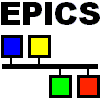
\includegraphics[width=3cm]{logo101}
}
\date{R3.14.4 Version,\\ \today.}
\maketitle
\newpage

\pagestyle{empty}

\section*{Involvements}
Bob Dalesio designed of original index file, data file layout,
and implemented the first prototype.\\
From then on, the following people have been involved at one
time or another:\\
\begin{center}
Thomas Birke,\\
Sergei Chevtsov,\\
Kay-Uwe Kasemir,\\ 
Chris Larrieu,\\
Craig McChesney,\\
Peregrine McGehee,\\
Nick Pattengale.
\end{center}

\section*{No Warranty}
Although the programs and procedures described in this manual are
meant to be helpful instruments for archiving, maintaining and
retrieving control system data, there is no warranty, either expressed
or implied, including, but not limited to, fitness for a particular
purpose. The entire risk as to the quality and performance of the
programs and procedures is with you.  Should the programs or
procedures prove defective, you assume the cost of all necessary
servicing, repair or correction.

In no event will anybody, including the persons listed above, be
liable to you for damages, including any general, special, incidental
or consequential damages arising out of the use or inability to use
the programs (including but not limited to loss of data or data being
rendered inaccurate or losses sustained by you or third parties or a
failure of the programs to operate with any other programs).

\newpage

\pagenumbering{roman}
\tableofcontents
\newpage
\pagestyle{headings}
\pagenumbering{arabic}
\setcounter{page}{1}

\chapter{Overview}
The Channel Archiver is an archiving toolset for the Experimental Physics
and Industrial Control System, \INDEX{EPICS}~\cite{ANLweb}.
It can archive any value that is available via \INDEX{ChannelAccess}
(\INDEX{CA}), the EPICS network protocol~\cite{hill89}.
We use the term ``archiver'' whenever we refer to the collection of
programs which allow us to take samples, place them into some storage
and retrieve them again.

\section{Audience}
Casual users will probably only need to know how to run the ``Java Archive
Viewer'' program and read its online help ---
none of which is part of this manual, except for a brief glimpse in 
section \ref{sec:javaclient}.
They may refer to the background information in chapter
\ref{ch:background} for a general understanding of the archiver.

Engineers who configure archive engines will need to be familiar with
the fundamentals up to and including the ArchiveEngine description in
chapter \ref{sec:engine}. They also need to understand the Example
Setup, chapter \ref{ch:examplesetup}, unless their site uses a
different setup which is then described in site-specific
documentation.

If you are stuck with installing and maintaining the archiver at your
site, you have to read and memorize this full document. Sorry. The table of
contents and index are meant to help, but you probably have to read it
once cover to cover.

\section{Channel Archiver Toolset}
The archiver toolset roughly splits into the following pieces:

\begin{description}
\item[\sffamily Sampling:]
The ArchiveEngine collects data from a given list of ChannelAccess
Channels.  The details of when a sample is taken etc.\ can be
configured: One may store every change, store changes that exceed a
dead band (that is configured on the CA server) or use periodic
scanning.
The configuration and operation of the ArchiveEngines will obviously
require some planning, as only data that was sampled and stored will
be available for future retrieval and analysis. Some sensible
compromise will have to be made between the urge to store all
miniscule changes of all the available channels at a site on one hand,
and data storage constraints on the other.

\item[\sffamily Storage:]
The data is stored in binary index and data files. Most end users need not
be concerned about the internals of those files, not even where they
are located, because additional indices allow several sub-archives to
appear like one, bigger, combined archive.
Somebody at each site, though, will need to perform maintenance
tasks: Decide where the data sets are located, how they are
backed up and how users can access them. 

\item[\sffamily Retrieval:]
The archiver toolset provides generic retrieval tools for browsing the
available channels and values, including simple multi-channel
comparisons.
An API allows users to write more sophisticated data analysis tools,
including an XML-RPC based network protocol for remote clients.
\end{description}


\chapter{Background}

\section{What is a Channel?} % -----------------------------------------------
The Channel Archiver deals with Channels that are served by EPICS
ChannelAccess. It stores all the information available via ChannelAccess:
\begin{itemize}
\item Time Stamp
\item Status/Severity
\item Value
\item Meta information:\\
      Units, Limits, ... for numeric channels,
      enumeration strings for enumerated channels.
\end{itemize}

\noindent The archiver stores the original \INDEX{time stamps} as it receives
them from ChannelAccess. It cannot check if these time stamps are valid, except
that it refuses to go ``back in time'' because it can only append new
values to the end of the data storage. It is therefore imperative to
properly configure the data sources, that is: the clocks on the CA
servers.

\label{back:in:time}
\NOTE If the CA server provides bad time stamps, for example stamps
that are older than values which are already in the archive, or stamps
that are unbelievably far ahead in the future, the ArchiveEngine will log
a warning message and refuse to store the affected samples.
This is a common reason for ``Why is there no data in my archive?''

As for the values themselves, the native data type of the channel as
reported by ChannelAccess is stored. For those familiar with the
ChannelAccess API, this means:
Channels that report a native data type of DBR\_xxx\_ are stored as
DBR\_TIME\_xxx after once requesting the full DBR\_CTRL\_xxx information.
 The Archiver can therefore handle scalar and array numerics
(double, int, ...), strings and enumerated types. 

\section{Data Sources} % -----------------------------------------------------
Before even considering the available \INDEX{sampling options}, it is
important to understand the \INDEX{data sources}, the \INDEX{ChannelAccess
servers} whose channels we intend to archive.
In most cases we will archive channels served by an EPICS Input/Output
Controller (\INDEX{IOC}) which is configured via a collection of EPICS
\INDEX{records}.
Alternatively, we can archive channels served by a custom-designed CA
server that utilizes the portable CA library \INDEX{PCAS}.
In those cases, one will have to contact the implementor of the custom
CA server for details.
In the following, we concentrate on the IOC scenario and use the
analog input record from listing~\ref{lst:airecord} as an example.

\lstinputlisting[float=htb,caption={``aiExample'' record},label=lst:airecord]{aiexample.db} 

\noindent What happens when we try to archive the channel ``aiExample''?
We will receive updates for the record's value field (VAL). In fact we
might as well have configured the archiver to use ``aiExample.VAL''
with exactly the same result.
The record is scanned at 10~Hz, so we can expect 10 values per second.
Almost: The archive deadband (ADEL) limits the values that we receive
via CA to changes beyond 0.1. When archiving this channel, we could
store at most 10 values per second or try to capture every change,
utilizing the ADEL configuration to limit the network traffic.

\NOTE The archiver has no knowledge of the scan rate nor the deadband
configuration of your data source! You have to consult the IOC
database or PCAS-based code to obtain these.

With each value, the archiver stores the time stamp as well as the
status and severity. For aiExample, we configured a high limit of 10
with a MAJOR severity. Consequently we will see a status/severity of
HIHI/MAJOR whenever the VAL field reaches the HIHI limit.
In addition to the value (VAL field), the archiver also stores certain
pieces of \INDEX{meta information}. For numeric channels, it will store the
engineering units, suggested display precision, as well as limits for
display, control, warnings, and alarms. For enumerated channels, it
stores the enumeration strings.
Applied to the aiExample record, the suggested display precision is
read from the PREC field, the limits are derived from HOPR, LOPR,
HIHI, ..., LOLO.

\NOTE You will have to consult the record reference manual or even
record source code to obtain the relations between record fields and
channel properties. The analog input record's EGU field for example
provides the engineering units for the VAL field. We could, however,
also try to archive aiExample.SCAN, that is the SCAN field of the same
record. That channel aiExample.SCAN will be an \emph{enumerated} type
with possible values ``Passive'', ``.1 second'' and so on. The EGU
field of the record no longer applies!
Another example worth considering: While HOPR defines the upper
control limit for the VAL field, what is the upper control limit if we
archive the HOPR field itself?

It is also important to remember that the archiver
--- just like any other ChannelAccess client --- does {\bfseries not} know
anything about the underlying EPICS record type of a channel. In fact
the channel might not be based on any record at all if we use a
PCAS-based server.
Given the name of an analog input record, it will store the record's
value, units and limits, that is: most of the essential record
information. Given the name of a stepper motor record, the
archiver will also store the record's value (motor position) with the
units and limits of the motor position. It will not store the
acceleration, maximum speed or other details that you might consider
essential parts of the record. To archive those, one would have to
archive them as individual channels.

\section{Sampling Options} % ---------------------------------------------
The ArchiveEngine supports these sampling mechanisms:
\begin{description}
\item[\sffamily Monitor:]
In this mode, the ArchiveEngine requests a CA monitor, i.e.\ it
subscribes to changes and we store all the values that the server
sends out. The CA server configuration determines when values are sent.

\item[\sffamily Sampled:]
In this mode, the ArchiveEngine periodically requests a value from
the CA server, e.g.\ every 30 seconds.

\item[\sffamily Sampled using monitors:]
This mode is very similar to the previous one:
The ArchiveEngine is again configured to store periodic samples,
e.g. one sample every 5 seconds. But instead of actively requesting a
value from the CA server at this rate, it establishes a monitor and
only saves a value every 5 seconds.
\end{description}

\noindent The difference between the two sampled modes is subtle but important
for performance reasons. Assume our data source changes at 1~Hz. If
we want to store a value every 30 seconds, it is most efficient to
send a 'read'-request every 30 seconds. If, on the other hand, we want
to store a value every 5 seconds, it is usually more effective to
establish a monitor, so we automatically receive updates about every
second, and simply ignore 4 of the 5 values.

When configuring a channel for the ArchiveEngine, the user only
selects either ``Monitor'' or provides a sampling rate.
The ArchiveEngine will automatically determine which mechanism to use
for sampled operation, periodic reads or monitors
(see get\_threshold configuration parameter for details).

\NOTE The values dumped into the data storage will not offer much
indication of the sampling method. In the end, we only see values with
time stamps. If for example the time stamps of the stored values
change every 20 seconds, this could be the result of a monitored
channel that happened to change every 20 seconds. We could also face a
channel that changed at 10~Hz but was only sampled every 20 seconds. 

\section{Time Stamps}
\begin{figure}[htb]
\begin{center}
\InsertImage{width=0.8\textwidth}{times}
\end{center}
\caption{\label{fig:times}Time Stamps and Sampling}
\end{figure}

Each ChannelAccess Server provides time-stamped data. An IOC for
example stamps each value when the corresponding record is
processed.  These time-stamps offer nano-second granularity. Most
applications will not require the full accuracy, but some
hardware-triggered acquisition, utilizing interrupts on a fast CPU,
might in fact put the full time stamp resolution to good use.

The ChannelArchiver as a generic tool does not know about the origin
of the time stamps, but it tries to conserve them.
Fig.~\ref{fig:times} shows the same channel, archived by different methods.
When using the ``Monitor'' method for archiving, we capture all the
changes of the channel, resulting in the data points marked by black
diamonds.
When we use scanned operation, e.g.\ every 1~second, the following
happens: About every second, the ArchiveEngine stores the current
value of the channel \emph{with its original time stamp!}.
So while the ArchiveEngine might take a sample at 10, 11, 12,
... seconds, it stores the time stamps that happen to come with the
values, and in this case those happened to be
9.9679712 seconds, 10.9894400 seconds, 11.7605488 seconds and so on.

\section{Sensible Sampling}
The data source configuration and sampling need to be coordinated.  In
fact the whole system needs to be understood. When we deal with water
tank temperatures as one example, we have to understand that the
temperature is unlikely to change rapidly. Let us assume that it only
varies within 30...60 seconds. The analog input record that reads the
temperature could be configured to scan every 2 seconds. Not because
we expect the temperature to change that quickly but mostly to provide
the operator with a warm and fuzzy feeling that we are still reading
the temperature: The operator display will show minuscule variations
in temperature every 2 seconds.  An ArchiveEngine that is meant to
capture the long-term trend of the tank temperature could then sample
the value every 60 seconds.

On the other extreme could be channels for vacuum readings along linac
cavities. The records that read them might be configured to scan as
fast as the sensing devices permit, maybe beyond 10~Hz, so that
interlocks on the IOC run as fast as possible. Their deadbands (ADEL
and MDEL) on the other hand are configured to limit the data rate that
is sent to monitoring CA clients: Only meaningful vacuum changes are
sent out, significantly reducing the amount of data sent onto the
network.  The ArchiveEngine can then be configured to monitor the
channel: During normal operation, when the vacuum is fairly stable, it
will only receive a few values, but whenever the vacuum changes
because of a leak, it will receive a detailed picture of the event.

Another example is a short-term archive that is meant to store
beam position monitor (BPM) readings for every beam pulse. The records
on the IOC can then be configured with ADEL=-1 and the ArchiveEngine
to use monitors, resulting in a value being sent onto the network and
stored in the archive even if the values did not change. The point
here is to store the time stamps and beam positions for each beam
pulse for later correlation. Needless to say that this can result in a
lot of data if the engine is kept running unattended. The preferred
mode of operation would be to run the engine only for the duration
of a short experiment.

\NOTE The scanning of the data source and the ArchiveEngine run in
parallel, they are not synchronized.
Example: If you have a record scanned every second and want to capture
every change in value, configuring the ArchiveEngine to scan every
second is {\bfseries not} advisable:
Though both the record and the ArchiveEngine would scan every
second, the two scans are not synchronized and rather unpredictable
things can happen. Instead, the "Monitor" option for the ArchiveEngine
should be used for this case.

\section{Time Stamp Correlation} 
\label{sec:timestampcorr}
We have stressed more than once that the Channel Archiver preserves
the original time stamps as sent by the CA servers.  This commonly
leads to difficulties when comparing values from different
channels. The following subsections investigate the issue in more
detail and show several ways of manipulating the data in order to
allow data reduction and cross-channel comparisons.

\subsection{``Raw'' Data}
Even when two channels were served by the same IOC, and originating from
records on the same scan rate, their time stamps will slightly differ
because a single CPU cannot scan several channels at exactly the same
time.  Tab.~\ref{tab:ABtimes} shows one example.

\begin{table}[htbp]
  \begin{center}
    \begin{minipage}[t]{0.49\textwidth}
      \begin{tabular}[t]{l|l}
        Time               & A         \\
        \hline
        17:02:28.700986000 & 0.0718241 \\
        17:02:37.400964000 & 0.0543581 \\
        ...
      \end{tabular}
    \end{minipage}%
    \begin{minipage}[t]{0.49\textwidth}
      \begin{tabular}[t]{l|l}
        Time               & B         \\
        \hline
        17:02:28.701046000 & -0.086006 \\
        17:02:37.510961000 & -0.111776 \\
        ...
      \end{tabular}
    \end{minipage}%
    \caption{Example Time Stamps for two Channels A and B.}
    \label{tab:ABtimes}
  \end{center}
\end{table}

\noindent When we try to export this data in what we call \INDEX{raw
spreadsheet format}, a problem arises: Even though the two channels'
time stamps are close, they do not match, resulting in a spreadsheet
as shown in Tab.~\ref{tab:ABraw}. Whenever one channel has a value,
the other channel has none and vice versa.  This spreadsheet does
not yield itself to further analysis; calculations like $A-B$ will
always yield \INDEX{'\#N/A'} since either A or B is undefined.

\begin{table}[htbp]
  \begin{center}
    \begin{tabular}[t]{l|l|l}
      Time                         & A         & B         \\
      \hline
      3/22/2000 17:02:28.700986000 & 0.0718241 & ---       \\
      3/22/2000 17:02:28.701046000 & ---       & -0.086006 \\
      3/22/2000 17:02:37.400964000 & 0.0543581 & ---       \\
      3/22/2000 17:02:37.510961000 & ---       & -0.111776 \\
      ...
    \end{tabular}
    \caption{Spreadsheet for raw Channels A and B.}
    \label{tab:ABraw}
  \end{center}
\end{table}

\subsection{Staircase Interpolation}
There are several ways of mapping channels onto matching time
stamps. One is what we call \INDEX{Staircase Interpolation} or
\INDEX{Filling}: Whenever there is no current value for a channel, we
re-use the previous value. This is often perfectly acceptable because
the CA server will only send updates whenever a channel changes
beyond the configured deadband. So if we monitored a channel and did
not receive a new value, this means that the previous value is still
valid --- at least within the configured deadband. In the case of
scanned channels we have no idea how a channel behaved in between
scans, but if we e.g.\ look at water temperatures, it might be safe to
assume that the previous value is still ``close enough''.
Table~\ref{tab:ABstair} shows the previously discussed data subjected
to staircase interpolation. Note that in this example there is no
initial value for channel B, resulting in one empty spreadsheet
cell. From then on, however, there are always values for both
channels, because any missing samples are filled by repeating the
previous one.

\NOTE While table~\ref{tab:ABstair} marks the filled values by
printing them in italics, spreadsheets generated by archive retrieval
tools will not accent the filled values in any way, so care must be
taken: Those filled values carry artificial time stamps. If you depend
on the original time stamps in order to synchronize certain events,
you must not use any form of interpolation but always retrieve the raw
data. 

\begin{table}[htbp]
  \begin{center}
    \begin{tabular}[t]{l|l|l}
      Time                         & A         & B         \\
      \hline
      3/22/2000 17:02:28.700986000 & 0.0718241 & ---       \\
      3/22/2000 17:02:28.701046000 & \textit{0.0718241}      & -0.086006 \\
      3/22/2000 17:02:37.400964000 & 0.0543581 & \textit{-0.086006} \\
      3/22/2000 17:02:37.510961000 & \textit{0.0543581} & -0.111776 \\
      ...
    \end{tabular}
    \caption{Spreadsheet for Channels A and B with Staircase
      Interpolation; ``filled'' values shown in italics.}
    \label{tab:ABstair}
  \end{center}
\end{table}

You did of course notice that the staircase interpolation does not
reduce the amount of data. Quite the opposite: In the above examples,
channels A and B each had 2 values. With staircase interpolation, we
don't get a spreadsheet with 2 lines of data but 4 lines of data.  The
main advantage of filling lies is the preservation of original time stamps.

\subsection{Linear Interpolation}
Linear interpolation generates artificial values from the raw
data. This can be used to reduce the amount of data: For a summary of
the last day, it might be sufficient to look at one value every 30
minutes, even though the archive could contain much more data.
Another aspect is partly cosmetic and partly a matter of convenience:
When we look at Tab.~\ref{tab:ABstair}, we find rather odd looking
time stamps. While these reflect the real time stamps that the
ArchiveEngine received from the ChannelAccess server, it is often
preferable to deal with data that has time stamps which are nicely
aligned, for example every 10 seconds: 11:20:00, 11:20:10, 11:20:20,
11:20:30 and so on.

\begin{figure}[htb]
\begin{center}
\medskip
\InsertImage{width=\textwidth}{interpol}
\end{center}
\caption{\label{fig:interpol}Linear Interpolation and Averaging, see text.}
\end{figure}

\noindent When we select ``Linear Interpolation'', the archive retrieval code
will actually automatically switch between three types of
interpolation: \INDEX{Linear Interpolation}, \INDEX{Averaging} and the
Staircase Interpolation that we already presented in the preceeding
subsection. All methods will modify the original time stamps and data
in order to transform them onto the requested periodic time stamps.  

In the following, refer to fig.~\ref{fig:interpol}, and compare the
raw samples shown in there with the result of interpolation.  When
linear interpolation onto e.g.\ multiples of 10 seconds is requested,
the following happens for each interval or ``time slot'' of 10 seconds
within the queried time range:
\begin{itemize}
\item If there was up to one scalar value of type double,
  long, int or short, either inside or preceding the current time
  slot, followed by at least one value after the current time slot,
  linear interpolation is used to determine the approximate value at
  the end of the time slot. Special values like ``Disconnected'' or
  ``Archiver Off'', that is samples that have no numeric data, are not
  interpolated.

  Most of the red squares in fig.~\ref{fig:interpol} exemplify this
  behavior: For time slots 11:20:00, 11:20:10, 11:20:20, ..., 11:21:10
  there is always exactly one raw value before and after the time
  slot, so linear interpolation is used to determine the approximate
  value at the time slots.
  The red squares do in fact exactly fall onto the connecting lines
  between raw samples if you consider the full time stamps, but the
  plotting program chosen to produce fig.~\ref{fig:interpol} rounds
  down to full seconds.
  The gap from 11:21:10 to 11:21:40 results from ``Disconnected''
  samples in the gap which cannot be interpolated.

\item Averaging is used if several values fall into the
  current time slot and the data type allows averaging,
  i.e.\ it's a scalar double, long, int or short.
  In this case, the retrieval reports the average over
  the values in the current time slot. For a time stamp
  it uses the center of the time slot.

  The blue and green stars in fig.~\ref{fig:interpol} result from
  averaging: Since more than one sample falls into the time slots
  which are 30 respectively 60 seconds wide, those samples are
  averaged and the resulting value for e.g.\ 60 second interpolation
  is reported in the middle of the 60-second time slots: 11:20:30, 11:21:30,
  11:22:30, etc. Note that the averaging also covers time slots that
  contain special non-values like the slot from 11:21:00 to 11:22:00:
  While there is a ``disconnected'' region in there, the remaining 5
  raw samples are used for averaging.

\item As a fallback, staircase interpolation is used for arrays or
  scalars of type string, char or enumerated, or when the single
  preceedign and following sample is a non-value like ``disconnected''
  or ``archiver off''. In short: cases that prohibit linear
  interpolation and averaging.  Staircase means in this case that the
  last value before a time slot is extrapolated onto the time slot.
  That's usually valid because we either sampled a slow changing
  channel, so the previous value is still good enough; or we archived
  on change and no change means the previous data is still valid.
  (While in fact one could interpolate or average certain arrays, we
  don't because for one that's expensive. In addition, EPICS arrays
  often contain more than just waveform elements: They're
  used to transfer structures.)
\end{itemize}


% interpol.tex
\section{Time Stamp Correlation} \label{sec:timestampcorr}
We have stressed more than once that the Channel Archiver preserves
the original time stamps as sent by the CA servers.  This commonly
leads to difficulties when comparing values from different
channels. The following subsections investigate the issue in more
detail and show several ways of manipulating the data in order to
allow data reduction and cross-channel comparisons.
In short, the options described in the following subsections are:
\begin{description}
\item[\sffamily Raw Data:]
  Provides every archived sample ``as is''.
\item[\sffamily Staircase/Filling:]
  Duplicates samples to form a spreadsheet.
\item[\sffamily Linear/Averaged Interpolation:]
  Provides exactly the requested number of data points by
  interpolating or averaging the raw samples.
\item[\sffamily Plot Binning:]
  Reduces the number of samples for plotting.
\end{description}

\subsection{``Raw'' Data} \label{sec:rawdata}
Even when two channels were served by the same IOC, and originating from
records on the same scan rate, their time stamps will slightly differ
because a single CPU cannot scan several channels at exactly the same
time.  Tab.~\ref{tab:ABtimes} shows one example.

\begin{table}[htbp]
  \begin{center}
    \begin{minipage}[t]{0.49\textwidth}
      \sffamily
      \begin{tabular}[t]{l|l}
        Time               & A         \\
        \hline
        17:02:28.700986000 & 0.0718241 \\
        17:02:37.400964000 & 0.0543581 \\
        ...
      \end{tabular}
    \end{minipage}%
    \begin{minipage}[t]{0.49\textwidth}
      \sffamily
      \begin{tabular}[t]{l|l}
        Time               & B         \\
        \hline
        17:02:28.701046000 & -0.086006 \\
        17:02:37.510961000 & -0.111776 \\
        ...
      \end{tabular}
    \end{minipage}%
    \caption{Example Time Stamps for two Channels A and B.}
    \label{tab:ABtimes}
  \end{center}
\end{table}

\noindent When we try to export this data in what we call \INDEX{raw
spreadsheet format}, a problem arises: Even though the two channels'
time stamps are close, they do not match, resulting in a spreadsheet
as shown in Tab.~\ref{tab:ABraw}. Whenever one channel has a value,
the other channel has none and vice versa.  This spreadsheet does
not yield itself to further analysis; calculations like $A-B$ will
always yield \INDEX{'\#N/A'} since either A or B is undefined.

\begin{table}[htbp]
  \begin{center}
    \sffamily
    \begin{tabular}[t]{l|l|l}
      Time                         & A         & B         \\
      \hline
      3/22/2000 17:02:28.700986000 & 0.0718241 & ---       \\
      3/22/2000 17:02:28.701046000 & ---       & -0.086006 \\
      3/22/2000 17:02:37.400964000 & 0.0543581 & ---       \\
      3/22/2000 17:02:37.510961000 & ---       & -0.111776 \\
      ...
    \end{tabular}
    \caption{Spreadsheet for raw Channels A and B.}
    \label{tab:ABraw}
  \end{center}
\end{table}

\subsection{``Before or at'' Interpretation of Start Times}
 \label{sec:starttime}
When you invoke a retrieval tool with a certain start time, the
archive will rarely contain a sample for that exact start time. As an
example, you might ask for a start time of ``07:00:00'' on some date. Not
because you expect to find a sample with that exact time stamp, but
because you want to look at data from the beginning of that day's
operations shift, which nominally began at 7am.

The software underlying all retrieval tools anticipates this scenario
by interpreting all start times as ``before or at''. Given a start time
of ``07:00:00'', it returns the last sample before that start
time, unless an exact match is found. So in case a sample for the
exact start time exists, it will of course be returned. But if the
archive contains no such sample, the previous sample is returned.

Applied to Tab.~\ref{tab:ABraw}, channel A, you would get the samples
shown in there not only if you asked for ``17:02:28.700986000'', the
exact start time, but also if you asked for ``17:02:30''.
It is left to the end user to decide whether that previous sample is
still useful at the requested start time, if it's ``close enough'', or
if it needs to be ignored.

\subsection{Staircase Interpolation/Filling} \label{sec:filling}
There are several ways of mapping channels onto matching time
stamps. One is what we call \INDEX{Staircase Interpolation} or
\INDEX{Filling}: Whenever there is no current value for a channel, we
re-use the previous value. This is often perfectly acceptable because
the CA server will only send updates whenever a channel changes beyond
the configured deadband. So if we monitored a channel and did not
receive a new value, this means that the previous value is still valid
--- at least within the configured deadband. In the case of scanned
channels we have no idea how a channel behaved in between scans, but
if we e.g.\ look at water temperatures, it might be safe to assume
that the previous value is still ``close enough''.
Table~\ref{tab:ABstair} shows the previously discussed data subjected
to staircase interpolation. Note that in this example there is no
initial value for channel B, resulting in one empty spreadsheet
cell. From then on, however, there are always values for both
channels, because any missing samples are filled by repeating the
previous one.  Because of the interpretation of start times explained
in section \ref{sec:starttime}, you would get the result in
 Tab.\ \ref{tab:ABstair} not only if you asked for values beginning
``3/22/2000 17:02:28.700986000'', but also when you asked for
e.g. ``17:02:30'': Since neither channel A nor B have a sample for that
exact time stamp, the retrieval library would select the
preceding sample for each channel, resulting in the output shown in 
Tab.\ \ref{tab:ABstair}.

\NOTE While table~\ref{tab:ABstair} marks the filled values by
printing them in italics, spreadsheets generated by archive retrieval
tools will not accent the filled values in any way, so care must be
taken: Those filled values carry artificial time stamps. If you depend
on the original time stamps in order to synchronize certain events,
you must not use any form of interpolation but always retrieve the raw
data. 

\begin{table}[htbp]
  \begin{center}
    \sffamily
    \begin{tabular}[t]{l|l|l}
      Time                         & A         & B         \\
      \hline
      3/22/2000 17:02:28.700986000 & 0.0718241 & ---       \\
      3/22/2000 17:02:28.701046000 & \textit{0.0718241}      & -0.086006 \\
      3/22/2000 17:02:37.400964000 & 0.0543581 & \textit{-0.086006} \\
      3/22/2000 17:02:37.510961000 & \textit{0.0543581} & -0.111776 \\
      ...
    \end{tabular}
    \caption{Spreadsheet for Channels A and B with Staircase
      Interpolation; ``filled'' values shown in italics.}
    \label{tab:ABstair}
  \end{center}
\end{table}

You did of course notice that the staircase interpolation does not
reduce the amount of data. Quite the opposite: In the above examples,
channels A and B each had 2 values. With staircase interpolation, we
don't get a spreadsheet with 2 lines of data but 4 lines of data.  The
main advantage of filling lies is the preservation of original time stamps.

\subsection{Linear/Averaged Interpolation}  \label{sec:lininterpol}
Linear interpolation generates artificial values from the raw
data. This can be used to reduce the amount of data: For a summary of
the last day, it might be sufficient to look at one value every 30
minutes, even though the archive could contain much more data.
Another aspect is partly cosmetic and partly a matter of convenience:
When we look at Tab.~\ref{tab:ABstair}, we find rather odd looking
time stamps. While these reflect the real time stamps that the
ArchiveEngine received from the ChannelAccess server, it is often
preferable to deal with data that has time stamps which are nicely
aligned, for example every 10 seconds: 11:20:00, 11:20:10, 11:20:20,
11:20:30 and so on.

\begin{figure}[htb]
\begin{center}
\medskip
\InsertImage{width=\textwidth}{interpol}
\end{center}
\caption{\label{fig:interpol}Linear Interpolation and Averaging, see text.}
\end{figure}

\noindent When we select ``Linear Interpolation'', the archive retrieval code
will actually automatically switch between three types of
interpolation: \INDEX{Linear Interpolation}, \INDEX{Averaging} and the
Staircase Interpolation that we already presented in the preceding
subsection. All methods will modify the original time stamps and data
in order to transform them onto the requested periodic time stamps.  

In the following, refer to fig.~\ref{fig:interpol}, and compare the
raw samples shown in there with the result of interpolation.  When
linear interpolation onto e.g.\ multiples of 10 seconds is requested,
the following happens for each interval or ``time slot'' of 10 seconds
within the queried time range:
\begin{itemize}
\item If there was up to one scalar value of type double,
  long, int or short, either inside or preceding the current time
  slot, followed by at least one value after the current time slot,
  linear interpolation is used to determine the approximate value at
  the end of the time slot. Special values like ``Disconnected'' or
  ``Archiver Off'', that is samples that have no numeric data, are not
  interpolated.

  Most of the red squares in fig.~\ref{fig:interpol} exemplify this
  behavior: For time slots 11:20:00, 11:20:10, 11:20:20, ..., 11:21:10
  there is always exactly one raw value before and after the time
  slot, so linear interpolation is used to determine the approximate
  value at the time slots.
  The red squares do in fact exactly fall onto the connecting lines
  between raw samples if you consider the full time stamps, but the
  plotting program chosen to produce fig.~\ref{fig:interpol} rounds
  down to full seconds.
  The gap from 11:21:10 to 11:21:40 results from ``Disconnected''
  samples in the gap which cannot be interpolated.

\item Averaging is used if several values fall into the
  current time slot and the data type allows averaging,
  i.e.\ it's a scalar double, long, int or short.
  In this case, the retrieval reports the average over
  the values in the current time slot. For a time stamp
  it uses the center of the time slot.

  The blue and green stars in fig.~\ref{fig:interpol} result from
  averaging: Since more than one sample falls into the time slots
  which are 30 respectively 60 seconds wide, those samples are
  averaged and the resulting value for e.g.\ 60 second interpolation
  is reported in the middle of the 60-second time slots: 11:20:30, 11:21:30,
  11:22:30, etc. Note that the averaging also covers time slots that
  contain special non-values like the slot from 11:21:00 to 11:22:00:
  While there is a ``disconnected'' region in there, the remaining 5
  raw samples are used for averaging.

\item As a fallback, staircase interpolation is used for arrays or
  scalars of type string, char or enumerated, or when the single
  preceding and following sample is a non-value like ``disconnected''
  or ``archiver off''. In short: cases that prohibit linear
  interpolation and averaging.  Staircase means in this case that the
  last value before a time slot is extrapolated onto the time slot.
  That's usually valid because we either sampled a slow changing
  channel, so the previous value is still good enough; or we archived
  on change and no change means the previous data is still valid.
  (While in fact one could interpolate or average certain arrays, we
  don't because for one that's expensive. In addition, EPICS arrays
  often contain more than just waveform elements: They're
  used to transfer structures.)
\end{itemize}

\subsection{Plot-Binning} \label{sec:plotbinning}
This method is meant for plotting, providing data that --- when
plotted --- looks exactly like the raw data, albeit significantly
reducing the number of data points and hence speeding up the plot.  To
accomplish this, the data is binned. For example, the time span of one
day, 24~hours, can be divided into 800 sections, each of which covers 108
seconds. Each of those sections is called a ``Bin''. The raw samples
for the day are then investigated as follows:
\begin{itemize}
\item If there is no sample for the time span of a bin, the bin
  remains empty.
\item If there is one sample, it is placed in the bin.
\item If there are two samples, they are placed in the bin.
\item If there are more than two samples, the first and last one
  are placed in the bin. In addition, two artificial samples are
  created with a time stamp right between the first and last sample.
  One contains the minimum, the other the maximum of all raw samples
  who's time stamps fall into the bin. They are presented to the user
  in the sequence initial, minimum, maximum, final.
\end{itemize}

Note that the ``before or at'' interpretation of start times does not
apply for Plot-Binning: The exact start time of the request is used
to determine the beginning of the first bin, and only samples within
each bin are considered, there is no interpolation onto bin-boundaries.
In general, the use of $N$ bins can result in up to 4$N$ data points,
since each bin might provide an initial, minimum, maximum and final value.
In most cases, this results in a significant data
reduction. As long as we plot this such that the width of the plot in
pixes is close to the number of bins, there is no visual difference
between the raw data plot and the binned plot.  Typical numbers for
$N$ are around the width of a computer screen in pixels, that is
800\ldots 1200.  For the special case were 3 raw values happen to fall
into every bin, we will get 4$N$ instead of 4$N$ data points. For
typical $N$, that is a slight but not dramatic increase in retrieval
or plotting time. It is neglectable compared to the fact that binning
guarantees an upper limit of 4$N$ data points, no matter how many raw
samples there are.


\chapter{\INDEX{ArchiveEngine}} \label{sec:engine}

\begin{figure}[htb]
\begin{center}
\InsertImage{width=\textwidth}{engine}
\end{center}
\caption{\label{fig:engine}Archive Engine, refer to text.}
\end{figure}

\noindent The ArchiveEngine is an EPICS ChannelAccess client. It can
save any channel served by any ChannelAccess server. One ArchiveEngine
can archive data from more than one CA server. For more details on the
CA server data sources, refer to section \ref{sec:datasource} on page
\pageref{sec:datasource}.  The ArchiveEngine supports the sampling
options that were described in section \ref{sec:sampling} on page
\pageref{sec:sampling}.  The ArchiveEngine is configured with an XML
file that lists what channels to archive and how. Each given channel
can have a different periodic scan rate or be archived in monitor mode
(on change).  One design target was: Archive 10000 values per second,
be it 1000 channels that change at 10Hz each or 10000 channels which
change at 1Hz.

The ArchiveEngine saves the full information available via
ChannelAccess: The value, time stamp and status as well as
control information like units, display and alarm limits, ...  
The data is written to an archive in the form of local disk files,
specifically index and data files.  Chapter \ref{chap:storage}
provides details on the file formats.
While running, status and configuration of the ArchiveEngine are
accessible via a built-in web server, accessible via any web browser
on the network.  The chapter on data retrieval, beginning on page
\pageref{chap:retrieval}, introduces the available retrieval tools
that allow users to look at the archived data.

\section{Configuration} \label{sec:engineconfig}
The ArchiveEngine expects an XML-type configuration file that follows
the document type description format from listing
\ref{lst:engineconfigdtd} (see section \ref{sec:dtdfiles} on DTD file
installation). Listing \ref{lst:engineconfigex} provides an
example. In the following subsections, we describe the various XML
elements of the configuration file.

\lstinputlisting[float=htb,keywordstyle=\sffamily,caption={XML DTD for
    the Archive Engine
    Configuration},label=lst:engineconfigdtd]{../Engine/engineconfig.dtd}

\lstinputlisting[float=htb,keywordstyle=\sffamily,caption={Example
    Archive Engine Configuration},label=lst:engineconfigex]{../Engine/engineconfig.xml}

\clearpage

\subsection{\INDEX{write\_period tag}}
This is a \INDEX{global option} that needs to precede any group and
channel definitions.  It configures the write period of the Archive
Engine in seconds. The default value of 30 seconds means that the
engine will write to Storage every 30 seconds.

\subsection{\INDEX{get\_threshold tag}} \label{sec:getthreshold}
This global option determines when the archive engine switches from
``Sampled'' operation to ``Sampled using monitors'' as described in
section \ref{sec:sampling}. Defaults to 20 seconds.

\subsection{\INDEX{file\_size tag}}
This global option determines when the archive engine will create a
new data file. The default of 100 means that the engine will continue
to write to a data file until that file reaches a size of
approximately 100~MB, at which point a new data file is created.

\subsection{\INDEX{ignored\_future tag}}
Defines ``too far in the future'' as ``now $+$ ignored\_future''. It
is specified in hours, and samples with time stamps beyond that time
are ignored.
Details: For strange reasons, the Engine sometimes receives values with invalid
time stamps. The most common example is a ``Zero'' time stamp: After
an IOC reboots, all records have a zero time stamp until they are
processed. For passive records, as commonly used for operator input,
this time stamp will stay zero until someone enters a value on an
operator screen or via a safe/restore utility. The Engine cannot
archive those values because the retrieval relies on the values being
sorted in time. A zero time stamp does not fit in.

Should an IOC (for some unknown reason) produce a value with an
outrageous time stamp, e.g. "1/2/2035", another problem occurs: Since
the archiver cannot go back in time, it cannot add further values to
this channel until the date "1/2/2035" is reached.  Consequently,
future time stamps have to be ignored. (default: 6h)

\subsection{\INDEX{buffer\_reserve tag}} \label{sec:reserve}
To buffer the samples between writes to the disk, the engine keeps a
memory buffer for each channel. The size of this buffer is rounded up
to the next integer from
$$ buffer\_reserve \times \frac{write\_period}{scan\_period}
$$ Since writes can be delayed by other tasks running on the same
computer as well as disk activity etc., the buffer is bigger than the
minimum required: buffer\_reserve defaults to 3.

\subsection{\INDEX{max\_repeat\_count tag}} \label{sec:repeats}
When sampling in a scanned mode (as opposed to monitored), the engine
stores only new values. As long as a value matches the preceding
sample, it is not written to storage. Only after the value changes, a
special value marked with a severity of ARCH\_REPEAT and a status that
reflects the number of repeats is written, then the new sample is
added.

This procedure conserves disk space. The disadvantage lies in the fact
that one does not see any new samples in the archive until the
channel changes, which can be disconcerting to some users. Therefore
the max\_repeat\_count configuration parameter was added. It forces
the engine to write a sample even if the channel has not change after
the given number of repeats. The default is 120, meaning that a
channel that is scanned every 30 seconds will be written once an hour
even if it had not changed. 

\subsection{\INDEX{disconnect tag}} \label{sec:disconnect}
This global option selects how ``disabled'' channels (see
\ref{sec:disable}) are handled. By default, disabled channels will
stay connected via ChannelAccess, but no values are archived.
When setting the ``disconnect'' option, disabled channels will instead
disconnect from ChannelAccess and then, later, attempt to reconnect
once the channel is again enabled.

In general, it is a good idea to stay with the default. That way we
leave the connection handling to the ChannelAccess client library,
which is optimized to do this. The engine will still receive new data,
and as soon as the channel is re-enabled, it can thus store the most
recent value.

The disconnect feature was added for the rare case that you have IOCs
that are temporarily off-line, and some PV will tell you about the
fact. You can then use that PV to disable and disconnect the affected
channels, preventing the ChannelAccess client library from continuing
to issue connection attempts. Another example would be that you want
to reduce the network load of continuing CA monitors for channels
that are archived via monitors at a high rate but disabled. 
Most likely, though, checking your channels' update rates or using a
temporary archive engine might be the better solution.

\subsection{\INDEX{group tag}}
Every channel belongs to a group of channels. The configuration file
must define at least one group. For organizational or aesthetic
purposes, you might add more groups. One important use of groups is
related to the ``disable'' feature, see section \ref{sec:disable}.

\subsubsection{\INDEX{name tag}}
This mandatory sub-element of a group defines its name.

\subsection{\INDEX{channel tag}}
This element defines a channel by providing its name and the sampling
options. A channel can be part of more than one group. To accomplish
this, simply list the channel as part of all the groups to which it
should belong.

\subsubsection{\INDEX{name tag}}
This mandatory sub-element of a channel defines its name. Any name
acceptable for ChannelAccess is allowed. The archive engine does not
perform any name checking, it simply passes the name on to the CA
client library, which in turn tries to resolve the name on the
network.  Ultimately, the configuration of your data servers decides
what channel names are available.

\subsubsection{\INDEX{period tag}} \label{sec:period}
This mandatory sub-element of a channel defines the sampling period.
In case of periodic sampling, this is the period at which the periodic
sampling attempts to operate. In case of monitored channels (see next
option), this is the estimated rate of change of the channel.
The period is specified in units of seconds.

If a channel is listed more than once, for example as part of
different groups, the channel will still only be sampled once. The
sampling mechanism is determined by maximizing the data rate. If, for
example, the channel ``X'' is once configured for periodic sampling
every 30 seconds and once as a monitor with an estimated period or one
second, the channel will in fact be monitored with an estimated period
of 1 second.

\subsubsection{\INDEX{scan tag}}
Either ``monitor'' or ``scan'' need to be provided as part of a
channel configuration to select the sampling method.  
True to its name, ``scan'' selects scanned operation, where the preceding
``period'' tag determines the sampling period, that is the time
between taking samples.
As an example, scanned operation with a period of 60 means: Every 60
seconds, the engine will write the most recent value of the channel to
the archive.

\subsubsection{\INDEX{monitor tag}}
As an alternative to the ``scan'' tag, ``monitor'' can be used,
requesting monitored operation, that is: An attempt is made to store
each change received via ChannelAccess. The ``period'' tag is used to
determine the in-memory buffer size of the engine. That means: If
samples arrive much more frequently than estimated via the ``period''
tag, the archive engine might drop samples. (See also
``buffer\_reserve'', \ref{sec:reserve}).


\subsubsection{\INDEX{disable tag}} \label{sec:disable}
This optional sub-element of a channel turns the channel into a
``disabling'' channel for the group. Whenever the value of the channel
is above zero, sampling of the whole group will be disabled until the
channel returns to zero or below zero
(see \ref{sec:disconnect} for additional disconnection).


This is useful for e.g.\ a group of channels related to power
supplies: Whenever the power supply is off, we might want to disable
scanning of the power supplies' voltage and current because those
channels will only yield noise. By disabling the sampling based on a
``Power Supply is Off'' channel, we can avoid storing those values
which are of no interest.

\NOTE There is no ``enabling'' feature, meaning: The channel
marked as ``disable'' will disable its group whenever it is above
zero. There is no ``enable'' flag that would enable archiving of a group
whenever the flagged channel is above zero.
If you want it the other way around, you typically add a CALC record
to handle the inversion.

\section{Example for Sampling}
Assuming that a channel ``fred'' actually emits monitors at 1~Hz,
these are examples for sampling it:
\begin{itemize}
\item ``fred 1 Monitor''\\
      Every value sent by fred is archived. Might be a good idea for
      some channels, but don't try to store every value of every PV
      of your control system indefinetely unless you are prepared to
      deal with that amount of data.

      Per default, the engine will write every 30 seconds. So it will
      have to allocate a buffer for about 30 samples, based on our
      estimate of 1 second between incoming monitors.
      With the default buffer\_reserve of 3, it will actually allocate
      a buffer for 60 values, so we don't loose data when the engine
      should get delayed in writing. On the other hand, when the
      computer is terribly busy, we might not receive any more values, either.
\item ``fred 1''\\
      The engine will sample once per second, and the channel changes
      once a second, so you might think that you archive every value
      just as in the previous example.  But think again. The sampling
      of the engine on the host and the scanning of the channel on the
      CA server are not synchronized, plus there are additional
      network delays. So you will sometimes miss values whenever more
      than one sample arrived between the engine's sampling, or get
      duplicate values whenever no new value arrived between the
      engine's sampling. Bad idea.

      Except: With the default get\_threshold of 20 seconds, the engine
      will not issue a 'get' every second. It will instead use a
      monitor, and ignore all data that arrives faster than one
      second. So this specific case will probably give the same result
      as the previous case.
\item ``fred 60''\\
      The engine will sample every 60 seconds. This is a very
      reasonable setup: The channel samples at 1 Hz, so you get
      frequent updates for the operator interface, but for the archive
      we only care about a sample per minute and save storage space by
      ignoring finer detail.

      With the default get\_threshold, that's it. If you changed the
      threshold to for example 70 seconds, the engine would use
      monitors, so it would receive the 1 Hz data and ignore 59
      samples each minute. That is probably a waste of network
      bandwidth. You might, on the other hand, get more consistent
      time stamps, since the '60 second' period is now based on the
      time stamps which the IOC sends, and not the host clock.
\item ``fred 10 Monitor''\\
      Probably an error. The engine is instructed to save every
      incoming monitor, but you told it to allocate buffers for only
      one value every 10 seconds, even though we knew that the channel
      will emit monitors much more often. So you will get ``overrun''
      errors, the engine will overwrite older samples in its ring
      buffer with newly arriving samples, and the archive will contain
      the last few samples that happened to be in the buffer at
      write-to-disk time.
\end{itemize}

\section{Starting and Stopping}
\subsection{Starting}
The ArchiveEngine is a command-line program that displays usage
information similar to the following:

\begin{lstlisting}[frame=none,keywordstyle=\sffamily]
ArchiveEngine Version 2.1.0, EPICS 3.14.4
 
USAGE: ArchiveEngine [Options] <config-file> <index-file>
 
Options:
  -port <port>         Web server TCP port
  -description <text>  description for HTTP display
  -log <filename>      write logfile
  -nocfg               disable online configuration
\end{lstlisting}

\noindent Minimally, the engine is therefore started by simply naming the
configuration file and the path to the index file, which can be in the
local directory:

\begin{lstlisting}[frame=none,keywordstyle=\sffamily]
ArchiveEngine engineconfig.xml ./index
\end{lstlisting}

\noindent After collecting some data, the ArchiveEngine will create the
specified index file together with data files in the same directory
that contains the index file.

\subsection{``-log'' Option}
This option causes the ArchiveEngine to create a log file into which
all the messages that otherwise only appear on the standard output are copied.

\subsection{``-description'' Option} \label{sec:enginedesc}
This option allows setting the description string that gets displayed
on the main page of the engine's built-in HTTP server, see
section \ref{sec:enginehttp}.

\subsection{``-port'' Option} \label{sec:engineport}
This option configures the TCP port of the engine's HTTP server, again
see section \ref{sec:enginehttp}. The default port number is 4812.

If you think this number stinks for a default, you are not too far off
base: In Germany, there is a very well known Au-de-Cologne called
4711.  Since forty-seven-eleven is therefore easily remembered by
anybody from Germany, adding 1 to each 47 and 11 naturally results in
an equally easy to remember 4812.
No, the archiver development is not funded by the 4711 company.

\subsection{``-nocfg'' Option}
This option disables the ``Config'' page of the engine's HTTP server,
in case you want to prohibit online changes.

\subsection{The ``archive\_active.lck'' File}
You can only run one ArchiveEngine per directory because it creates
the index and data files in there.  When running, this lock file is
created. The ArchiveEngine will refuse to run if this file already
exists.  After shutdown, the ArchiveEngine will remove this lock file.
If the ArchiveEngine crashes or is not stopped gracefully by the
operating system, this lock file will be left behind.  You cannot
start the ArchiveEngine again until you remove the lock file. This is
a reminder for you to check the cause of the improper shutdown and
maybe check the data files for corruption.

\NOTE This is no 100\%\ dependable check. Data corruption occurs when
two engines attempt to write to the same index and data files. The
lock file, however, is created in the directory where the
ArchiveEngine was started, which could be different from the directory
where the data gets written. Example:

\begin{lstlisting}[frame=none,keywordstyle=\sffamily]
cd /some/dir
ArchiveEngine -p 7654 engineconfig.xml /my/data/index &

cd /another/dir
ArchiveEngine -p 7655 engineconfig.xml /my/data/index &
\end{lstlisting}

\noindent This is a sure-fire way to corrupt the data in
``/my/data/index'' and the accompanying data files because two
ArchiveEngines are writing to the same archive.

\subsection{More than one ArchiveEngine}
You can run multiple ArchiveEngines on the same
computer. But they must
\begin{enumerate}
\item be in separate directories. See the preceding discussion of
      the lock file which is meant to assist in avoiding this
      problem.
\item use a different TCP port number for the built-in web server
\end{enumerate}
In practice this means that you have to create different directories
on the disk, one per ArchiveEngine, and in there run the
ArchiveEngines with different "-p $<$port$>$" options.

\subsection{Stopping}
While the ArchiveEngine can be stopped by pressing ``CTRL-C''
or using the equivalent ``kill'' command in Unix, the preferred method is
via the built-in web server. Use any web browser and point it to

\begin{lstlisting}[frame=none,keywordstyle=\sffamily]
http://<host where engine is running>:<port>/stop
\end{lstlisting}

\noindent Per default, the engine uses 4812, so you could use the
following URL to stop that engine on the local computer:

\begin{lstlisting}[frame=none,keywordstyle=\sffamily]
http://localhost:4812
\end{lstlisting}

% ---------------------------------------------------------------------------
\section{\INDEX{Engine Web Server}} \label{sec:enginehttp} % ----------------
\begin{figure}[htb]
\begin{center}
\InsertImage{width=0.8\textwidth}{engine_main}
\end{center}
\caption{\label{fig:engine:main}Main Page of Archive Engine's HTTPD}
\end{figure}

The ArchiveEngine has a built-in web server (HTTP Daemon) for status
and configuration information.  You can use any web browser to access
this web server.  You can do that on the computer where the
ArchiveEngine is running as well as from other computers, be it a PC
or Macintosh or other system as long as that computer can reach the
machine that is running the ArchiveEngine via the network.  You do
\emph{not} need a web server like the Apache web server for Unix or
the Internet Information Server for Win32 to use this. The
ArchiveEngine \emph{itself} acts as a web server.

You \emph{cannot} view archived data with this mechanism.  See the
documentation on data retrieval (chapter \ref{chap:retrieval}) for
that, because the archive engine's HTTPD is meant for access to the
status and configuration of the running engine, not for accessing the
data samples.

To access the ArchiveEngine's web server, you need to know the
Internet name of the machine that is running the ArchiveEngine as well
as the TCP port.  If you are on the same machine, use ``localhost''.
The port is configured when you start the ArchiveEngine, it defaults
to 4812. Then use any web browser and point it to

\begin{lstlisting}[frame=none,keywordstyle=\sffamily]
 http://<host where engine is running>:<port>
\end{lstlisting}

\noindent Example for an ArchiveEngine running on the local machine with the
default port number:

\begin{lstlisting}[frame=none,keywordstyle=\sffamily]
http://localhost:4812
\end{lstlisting}

\noindent The start page of the ArchiveEngine web server should look
similar to the one shown in Fig.~\ref{fig:engine:main}. By following
the links, one can investigate the status of the groups and channels
that the ArchiveEngine is currently handling. The ``Config'' page
allows limited online-reconfiguration. Whenever a new group or channel
is added, the engine attempt to write a new config file called
\INDEX{onlineconfig.xml} in the directory where is was started.
It is left to the user to decide what to do with this file: Should it
replace the original configuration file, so that online changes are
preserved? Or should it be ignored, because online changes are only
meant to be temporary and with the next run of the engine, the
original configuration file will be used?

Note also that the ArchiveEngine does not allow online removal of
channels and groups. The scan mechanism of a channel can only be
changed towards a higher scan rate or lower period, similar to the
handling of multiply defined channels in a configuration file. Refer
to the section discussing the ``period'' tag on page \pageref{sec:period}.

\section{Threads} % ----------------------------------------------------------
The ArchiveEngine uses several threads:
\begin{itemize}
\item A main thread that reads the initial configuration and then
  enters a main loop for the periodic scan lists and writes to the
  disk.
\item The ChannelAccess client library is used in its multi-threaded
  version. The internals of this are beyond the control of the
  ArchiveEngine, the total number of CA client threads is unknown.
\item The ArchiveEngine's HTTP (web) server runs in a separate thread,
  with each HTTP client connection again being handled by its own
  thread. The total number of threads therefore depends on the number
  of current web clients.
\end{itemize}
As a result, the total number of threads changes at runtime. Though
these internals should not be of interest to end users, this can be
confusing especially on older releases of Linux where each thread
shows up as a process in the process list.
On Linux version 2.2.17-8 for example we get process table entries as
shown in Tab.~\ref{lst:aeprocs} for a single ArchiveEngine, connected
to four channels served by excas, no current web client. The only hint
we get that this is in fact one and the same ArchiveEngine lies in the
consecutive process IDs.

\begin{lstlisting}[float=htb,
caption={Output of Linux 'ps' process list command, see text.},
label=lst:aeprocs]
  PID TTY          TIME CMD
29721 pts/5    00:00:00 ArchiveEngine
29722 pts/5    00:00:00 ArchiveEngine
29723 pts/5    00:00:00 ArchiveEngine
29724 pts/5    00:00:00 ArchiveEngine
29725 pts/5    00:00:00 ArchiveEngine
29726 pts/5    00:00:00 ArchiveEngine
29727 pts/5    00:00:00 ArchiveEngine
29728 pts/5    00:00:00 ArchiveEngine   
\end{lstlisting}

The first conclusion is that one should not be surprised to see
multiple ArchiveEngine entries in the process table.
The other issue arises when one tries to 'kill' a running
ArchiveEngine. Though the preferred method is via the engine's web
interface, one can try to send a signal to the first process, the one
with the lowest PID.


\chapter{ArchiveDaemon}
\begin{figure}[htb]
\begin{center}
\InsertImage{width=0.8\textwidth}{daemon}
\end{center}
\caption{\label{fig:daemon}Archive Daemon, refer to text.}
\end{figure}

\noindent The ArchiveDaemon is a script that automatically starts,
monitors and restarts ArchiveEngines on the local host. It includes a
built-in web server, so by listing all the ArchiveEngines that are
meant to run on a host in the ArchiveDaemon's configuration file, one
can check the status of all these engines on a single web page as
shown in Fig.~\ref{fig:daemon}.

The daemon will attempt to start any ArchiveEngine that it does not
find running. In addition, the daemon can periodically stop and
restart ArchiveEngines in order to create e.g.\ daily sub-archives.
Furthermore, it adds each sub-archive to a configuration file for the
ArchiveIndexTool and runs the latter, so that all the sub-archives can
be accessed as if they were one big archive.

Before attempting to use the ArchiveDaemon, one should be familiar
with the configuration of the ArchiveEngine (sec.\ \ref{sec:engine}),
and how to start and stop it. Furthermore, one needs to be familiar
with the ArchiveIndexTool (sec.\ \ref{sec:indextool}).

\subsection{Configuration}
The ArchiveDaemon expects to find a configuration file called
``ArchiveDaemon.xml'' in the directory where it is started.  That
configuration file, an example of which can be found in listing
\ref{lst:daemonconfigex}, needs to follow the DTD from listing
\ref{lst:daemonconfigdtd}.

\lstinputlisting[float=htb,keywordstyle=\sffamily,caption={Example Archive Daemon Configuration},label=lst:daemonconfigex]{../ArchiveDaemon/ArchiveDaemon.xml}

\lstinputlisting[float=htb,keywordstyle=\sffamily,caption={XML DTD for
    the Archive Daemon Configuration},label=lst:daemonconfigdtd]{../ArchiveDaemon/ArchiveDaemon.dtd}

\noindent The configuration lists all the
ArchiveEngines that the daemon should manage on the local
computer. One ``engine'' element per ArchiveEngine specifies the
configuration of each engines. Specifically, the following tags are
allowed:

\subsubsection{desc}
This mandatory element is used for the ``-description'' option of the
Archive Engine, see section \ref{sec:enginedesc}.

\subsubsection{port}
This mandatory element determines the port number of the engine's HTTP
server, see section \ref{sec:engineport}.

\NOTE The ArchiveDaemon itself requires a TCP port number for its HTTP
server. The port numbers used by the ArchiveDaemon and all the Archive
Engines need to be different. You cannot use the same port number more
than once per computer.

\subsubsection{config}
This mandatory element must contain the full path to the configuration
file of the respective ArchiveEngine, see section \ref{sec:engineconfig}.

\subsubsection{daily}
This optional element configures the ArchiveDaemon to restart the
ArchiveEngine periodically. The element must contain a time in the
format ``HH:MM'' with 24-hour hours HH and minutes MM. One example
would be ``02:00'' for a restart at 2~am each morning.

\subsection{Operation}
The ArchiveDaemon is a perl script that is typically started like this:

\begin{lstlisting}[keywordstyle=\sffamily]
$ cd whereever_you_placed_ArchiveDaemon.xml
$ perl ArchiveDaemon.pl
Read ArchiveDaemon.xml, will disassociate from terminal
and from now on only respond via
          http://localhost:4610
You can also monitor the log file:
          ArchiveDaemon.log
\end{lstlisting}

\noindent One can use any web browser to connect to the daemon's HTTP server
under the URL shown in the above status message. Fig.~\ref{fig:daemon}
shows one example. The ArchiveDaemon offers a command line option for
selecting a specific TCP port.
Whenever running more than one ArchiveDaemon per computer, they
need to be started with different TCP port numbers. Furthermore, each
ArchiveEngine needs a different TCP port number.
\begin{lstlisting}[keywordstyle=\sffamily]
USAGE: ArchiveDaemon [-p port] 
       -p <port> : TCP port number for HTTPD
\end{lstlisting}

\noindent The ArchiveDaemon will create or use the following files in the
directory in which it was started:
\begin{itemize}
\item ArchiveDaemon.log\\
  The log file of the ArchiveDaemon.
\item indexconfig.xml\\
  This is a configuration file for the ArchiveIndexTool.  If the file
  already exists, the ArchiveDaemon will add every new sub-archive
  that it creates to the file. If the file does not exist, one will be
  created the next time a new sub-archive is started.
\item ArchiveIndexTool.log\\
  The log file of the last run of the ArchiveIndexTool.
\item master\_index\\
  The ArchiveIndexTool is run with indexconfig.xml to update
  this master index file.
\end{itemize}

\noindent The ArchiveDaemon configuration file must list the full path
names to the configuration files for the ArchiveEngines.
Within each of those directories, an ArchiveEngine is run and the
following files will be created:
\begin{itemize}
\item ArchiveEngine.log\\
  A log file for the ArchiveEngine running in that directory
\item archive\_active.lck\\
  Lock file of the ArchiveEngine
\item YYYY/MM\_DD/index \\
  A subdirectory for index and data files of the sub-archive.  If the
  ArchiveDaemon is configured to perform daily restarts, the format
  uses the year, month and day to build the path name.
\end{itemize}


\chapter{Data Retrieval}  \label{chap:retrieval}
Data retrieval requirements can cover a wide range.  One person might
be interested in the temperature of a water tank during the last
night. For this, it is probably sufficient to retrieve the raw data
for the respective channel and plot it.  If, on the other hand, we
want to look at the same temperature for the last 3 month, the raw
data will amount to too many samples and some sort of data reduction
or interpolation is helpful.  We already mentioned the problems of
time stamp correlation that arise when comparing different channels in
section \ref{sec:timestampcorr}.

The Channel Archiver toolset includes some generic tools that can be
used ``as is''. While those try to cover many data retrieval
requirements, certain requests can only be handled in customized data
mining programs (which might be e.g.\ perl scripts). For this, the
archiver offers a network data server. In short, these are your
options:

\begin{itemize}
\item Java Archive Client\\
      This is meant to be \emph{the} data client. Use it to browse the
      available data, generate plots, export data to spreadsheets,
      from any computer on the network by accessing the network data server.
\item ArchiveExport\\
      A command-line tool. Less convenient to use, requires direct
      access to the data files. Use this when the Java Archive Client
      or network data server are not available.
\item Archive Data Server\\
      You can access the Archive Data Server via XML-RPC from most
      programming languages. Use this method for customized data
      mining programs.
\end{itemize}
\section{ArchiveExport}
ArchiveExport is a command-line tool for local tests, i.e. it does
\emph{not} connect to the archive data server but requires that
you have direct read access to the index and data files.
It is mostly meant for testing.

When invoked without valid arguments, it will display a command
description similar to this:

\begin{lstlisting}[frame=none,keywordstyle=\sffamily]
USAGE: ArchiveExport [Options] <index file> {channel}
 
Options:
  -verbose               Verbose mode
  -list                  List all channels
  -info                  Time-range info on channels
  -start <time>          Format:
                      "mm/dd/yyyy[ hh:mm:ss[.nano-secs]]"
  -end <time>            (exclusive)
  -text                  Include text column for
                         status/severity
  -match <reg. exp.>     Channel name pattern
  -interpolate <seconds> interpolate values
  -output <file>         output to file
  -gnuplot               generate GNUPlot command file
  -Gnuplot               generate GNUPlot output
                         for Image
\end{lstlisting}

\noindent ArchiveExport produces spreadsheet-type output in
TAB-separated ASCII text, suitable for import into most spreadsheet
programs for further analysis. Per default, ArchiveExport uses
Staircase Interpolation to map the data for the requested channels
onto matching time stamps, but one can select Linear Interpolation via
the ``-interpolate'' option. See section \ref{sec:timestampcorr} on
page~\pageref{sec:timestampcorr} for details.

Assuming that your current working directory contains an
archive index file that is aptly named ``index'', the following
invocation will generate a spreadsheet file ``data.txt'' with the data
of all channels that match the pattern ``IOC'' for the date of January
27, 2003:

\begin{lstlisting}[frame=none,keywordstyle=\sffamily]
ArchiveExport index -m IOC \
              -s "01/27/2003" \
              -e "01/28/2003" >data.txt
\end{lstlisting}

\noindent To plot this in OpenOffice, you could create a new
spreadsheet, then use the menu item Insert/Sheet/FromFile, select the
file ``data.txt'' and configure the text import dialog to use
``Separated by Tab''. You will notice that even though the original
text file contains time stamps with nano-second resolution, for
example ``01/27/2003 23:57:25.579346999'', the spreadsheet program
might use a default representation of e.g. 
``01/27/03 23:57 pm''.
In order to see the full time stamp detail, one needs to reformat
those spreadsheet columns with a user-defined format like
``MM/DD/YYYY HH:MM:SS.000000000''.
If you use Microsoft Excel, you might be limited to a format with
millisecond resolution: ``MM/DD/YYYY HH:MM:SS.000''.

For graphing the data, the most suitable option is often an
``X-Y-Graph'', using the first row for labels, with the data series
taken from the columns.

\section{Java Archive Client}
This tool is meant to be the main data retrieval tool. It provides a
graphical user interface to allow data browing. It is based on Java
and hence usable on many operating systems. It accesses the data via
the DataServer described in section \ref{sec:dataserver}, which means
that it can access the data via the network.

In short, it's the greatest thing since canned beer.
\clearpage
\section{Data Server} \label{sec:dataserver}
The archiver toolset includes a network data server.
By running this data server on a computer that has
physical access to your archived data, be it because the data resides
on a local disk or an NFS-mapped volume, other machines
on the network can get read-access to your data.

\begin{figure}[htb]
\begin{center}
\InsertImage{width=0.8\textwidth}{dataserver}
\end{center}
\caption{\label{fig:dataserver}Data Server, refer to text.}
\end{figure}

\noindent The data server uses XML-RPC to serve the data. This means that
software running on disparate operating systems, running in different
environments can access your data over the Internet. As an example,
your data server might be a Linux machine on a subnet behind a
firewall. After you configure the firewall to pass HTTP requests, any
Linux, Win32, Macintosh computer both inside or outside of the
firewall can access the data from within perl, python or tcl scripts,
programs written in C, C++ or Java, actually pretty much any programming
language. As illustrated in fig.~\ref{fig:dataserver}, the client
program sends its requests to a web server, which forwards it to the
data server. The dataserver accesses the relevant archives --- you
determine which ones are available via a configuration file --- and
returns the data though the web server to the client program.  You can
configure access security via e.g.~ the Apache web server
configuration because the data server is simply a CGI program.
XML-RPC handles the data type conversions. For details on how to use
XML-RPC from your code, refer to section \ref{sec:xmlprotocol} on page
\pageref{sec:xmlprotocol}.

\subsection{Installation} % ---------------------------------------------
After successful compilation in ChannelArchiver/XMLRPCServer, you will
have a program ``ArchiveDataServer''. You need to copy that binary as
``ArchiveDataServer.cgi'' into your web server's CGI directory and
assert that the web server can execute the ArchiveDataServer.
The ``.cgi'' extension is important, because otherwise your web server
might not recognize your CGI program as such.
What follows is an example setup for the Apache Web Server under Linux:
\begin{enumerate}
\item Check your Apache configuration file, which can often been found
  in ``/etc/httpd/conf/httpd.conf'', for the location of your cgi-bin
  directory.  In my case, there was already a CGI directory /var/www/cgi-bin.

\item Create a new CGI directory so that we can specifically configure
   it.\\
   Adding the following to the Apache config file worked for me:
\begin{lstlisting}[keywordstyle=\sffamily]
<Directory /var/www/cgi-bin/xmlrpc>
   SetEnv LD_LIBRARY_PATH  /usr/local/lib:...
   SetEnv SERVERCONFIG /var/www/cgi-bin/ \
                   xmlrpc/serverconfig.xml
</Directory>
\end{lstlisting}
  The LD\_LIBRARY\_PATH needs to include all the directories that
  contain shared libraries which your ArchiveDataServer.cgi uses.
  In many cases, this means the EPICS base and extensions' lib
  directories as well as the install location of the expat and XML-RPC
  libraries.
  The SERVERCONFIG variable needs to point to your server configuration
   file, more about which next.
\end{enumerate}

\subsection{Setup}
You need to prepare an XML-formatted configuration file for the
ArchiveDataServer that follows the DTD from listing
\ref{lst:serverconfigdtd}. Note that the ArchiveDataServer might not
verify your configuration file, so you are strongly encouraged to use a
tool like 'xmllint' on Linux to check your configuration against the
DTD. Listing \ref{lst:serverconfigex} shows one example
configuration which lists two archives to be served. Client programs
will internally use the respective 'key' to access them.

\lstinputlisting[float=htb,keywordstyle=\sffamily,caption={XML DTD for the Data Server Configuration},label=lst:serverconfigdtd]{../XMLRPCServer/serverconfig.dtd}
\lstinputlisting[float=htb,keywordstyle=\sffamily,caption={Example Data Server Configuration},label=lst:serverconfigex]{../XMLRPCServer/serverconfig.xml}

\clearpage
\section{XML-RPC Protocol} \label{sec:xmlprotocol}
The following is a description of the calls implemented by the archive
data server based on the XML-RPC protocol.
For details on XML-RPC,  including the specifications and examples of
how to use it from within C,  C++, Java, perl, please refer to
\href{http://www.xmlrpc.com}{http://www.xmlrpc.com}.

Users of Java should probably utilize the Java archive data client
library provided with the ChannelArchiver. Users of other programming
environments need to refer to the following.

\subsection{archiver.info} \label{sec:archiver:info} % ------------------- 
This call returns version information. It will allow future
compatibility if clients check for the correct version numbers.  In
addition, it provides hints on how to decode the values served by this
server.

\begin{lstlisting}[keywordstyle=\sffamily]
{ int32             ver,
  string            desc,
  string            how[],
  string            stat[],
  { int32 num,
    string sevr,
    bool has_value,
    bool txt_stat
  }                 sevr[]
 } = archiver.info()
\end{lstlisting}

\begin{description}
\item[\sffamily ver:]  Version number. The first released software uses '1'.
\item[\sffamily desc:] Cute description that one can print.
\item[\sffamily how:]  Array of strings with a description of the
                       request methods supported for 'how' in the
		       archiver.values() call described further below in
                       section \ref{sec:archiver:values}.
\item[\sffamily stat:] Array of strings with a description of the
                       ``status'' part of the values returned by
                       the archiver.values() call.     
\item[\sffamily sevr:] Array of structures with a description of the
                       ``severity'' part of the values returned by
                       the archiver.values() call.     
\end{description}

\noindent The result is a structure with a numeric ``ver''
member, a string ``desc'' member and so on as listed above.
Implementations like perl will return a hash with members
``ver'', ``desc'', etc.
The strings in ``how'' describe the request method for how=0, how=1,
and so on.
The strings in ``stat'' describe the enumerated status values, the
typical result is shown in table \ref{tab:stat}.

The more important information is in the ``sevr'' array.
It also lists severity numbers (``num'') and their associated string
representation (``sevr''). In addition to the alarm severities defined
by the EPICS base software, the archiver uses some special severity
values which have the ``has\_value'' property set to false. They
identify situations that have no value because the channel
was disconnected or the archiver was turned off. Other special
severities identify repeat counts which are used in the periodic
scanning modes of the archive engine: If the channel did not change
for N sample times, a repeat count of N is logged instead of logging
the same value N times. In that case, the ``txt\_stat'' property is
set to false because the status (stat) field no longer corresponds to
a status string from table \ref{tab:stat}. Instead, it provides the
repeat count N.
Table \ref{tab:sevr} lists the typical content of the ``sevr'' array,
table \ref{tab:statsevrexample} presents examples for decoding values
based on their status and severity information.

\begin{table}[htbp]
  \begin{center}
    \sffamily
    \begin{tabular}[t]{l|l}
    Array Element & String \\
    \hline
      0   & NO\_ALARM   \\
      1   & READ ALARM   \\
      2   & WRITE ALARM \\
      3   & HIHI ALARM  \\
      4   & HIGH ALARM  \\
      5   & LOLO ALARM  \\
      6   & LOW ALARM  \\
      7   & STATE ALARM  \\
      \ldots   & \ldots  \\
      17   & UDF ALARM  \\
      \ldots   & \ldots  \\
    \end{tabular}
    \caption{Alarm Status Values returned in the ``stat'' member of archiver.info()}
    \label{tab:stat}
  \end{center}
\end{table}

\begin{table}[htbp]
  \begin{center}
    \sffamily
    \begin{tabular}[t]{l|l|l|l}
     num & sevr             & has\_value & txt\_stat \\
    \hline
       0 & NO\_ALARM        & true       & true  \\
       1 & MINOR            & true       & true  \\
       2 & MAJOR            & true       & true  \\
       3 & INVALID          & true       & true  \\
    3968 & Est\_Repeat      & false      & false \\
    3856 & Repeat           & false      & false \\
    3904 & Disconnected     & false      & true  \\
    3872 & Archive\_Off     & false      & true  \\
    3848 & Archive\_Disabled& false      & true
    \end{tabular}
    \caption{Alarm Severity Values returned in the ``sevr'' member of archiver.info()}
    \label{tab:sevr}
  \end{center}
\end{table}

\begin{table}[htbp]
  \begin{center}
    \sffamily
    \begin{tabular}[t]{l|l|l|l}
    Severity (sevr) & Status (stat) & Value & Example Text \\
    \hline
                  0 &            0  &  3.14 & ``3.14'' \\
                  1 &            6  &  3.14 & ``3.14 MINOR LOW'' \\
               3856 &            6  &  3.14 & ``3.14 Repeat 6'' \\
               3904 &            0  &  0    & ``Disconnected'' \\
    \end{tabular}
    \caption{Examples for decoding samples returned from the
    archiver.values() call based on their Status and Severity}
    \label{tab:statsevrexample}
  \end{center}
\end{table}

\subsection{archiver.archives} % --------------------------------------------
Returns the archives that this data server can access.

\begin{lstlisting}[keywordstyle=\sffamily]
{ int32 key, 
  string name, 
  string path }[] = archiver.archives()
\end{lstlisting}

\begin{description}
\item[\sffamily key:] A numeric key that is used by the following
                      routines to select the archive.
\item[\sffamily name:] A description of the archive that one could
                       e.g.\ use in a drop-down selector in a GUI
                       application for allowing the user to select an archive.
\item[\sffamily path:] The path to the index file,  valid on the file
                       system where the data server runs.
                       It might be meaningful to a few users who want to
                       know exactly where the data resides,  but it is
                       seldom essential for XML-RPC clients to look at this.
\end{description}

\noindent The result is an array of structures with a numeric ``key''
member and strings ``name'' and ``path''.
An example result could be:
\begin{lstlisting}[keywordstyle=\sffamily]
{ key=1,  name="Vacuum", path="/home/data/vac/index" },
{ key=2,  name="RF",     path="/home/data/RF/index" }
\end{lstlisting}

\noindent So in the following one would then use key=1 to access
vacuum data etc. One can expect the keys to be small,  positive
numbers,  but they are not guaranteed to be consecutive as 1, 2, 3,
... Since the keys could be something like 10,  20, 30 or 1, 17, 42,
they are not useful as array indices.

\subsection{archiver.names} % ------------------------------------------
Returns channel names and start/end times.
The key must be a valid key obtained from archiver.keys.
Pattern is a regular expression;
if left empty,  all names are returned.

\NOTE The Time Stamps are \emph{not} the raw EPICS time stamps with 1990 epoch, 
but use the time\_t data type based on a 1970 epoch.

\begin{lstlisting}[keywordstyle=\sffamily]
{string name, 
 int32 start_sec,  int32 start_nano,
 int32 end_sec,    int32 end_nano}[] 
         = archiver.names(int32 key,  string pattern)
\end{lstlisting}

\noindent The result is an array of structures,  one structure
per channel that matches the pattern.
Start/end gives an idea of the time range that can
be found in the archive for that channel.
The archive might actually contain entries \emph{after}
the reported end time because the index might not
be up too date on the end times.

\subsection{archiver.values} \label{sec:archiver:values} % -----------------
This call returns values from the archive identified by the key for a
given list of channel names and a common time range.

\begin{lstlisting}[keywordstyle=\sffamily]
result = archiver.values(
         int key, 
         string name[], 
         int32 start_sec,  int32 start_nano,
         int32 end_sec,  int32 end_nano, int32 count,
         int32 how)
\end{lstlisting}

\noindent The parameter ''how'' determines how the raw values of the
various channels get arranged to meet the requested time range and
count.  For details on the methods mentioned in here refer to section
\ref{sec:timestampcorr} and following, beginning on page
\pageref{sec:timestampcorr}.
\begin{description}
\item[\sffamily how = 0 (raw):]
  Get raw data from archive (see \ref{sec:rawdata}), starting w/ 'start',
  up to either 'end' time or max. 'count' samples.
\item[\sffamily how = 1 (filled/staircase spreadsheet):]
  Get data that is filled or staircase-interpolated, starting
  w/ 'start', up to either 'end' time or max. 'count' samples
  (see \ref{sec:filling}).
  For each channel, the same number of values is returned. The
  time stamps of the samples match accross channels, so that one can
  print the samples for each channel as columns in a spreadsheet.
  If a spreadsheet cell is empty because the channel does not have any
  useful value for that point in time, a status/severity of
  UDF/INVALID is returned (Tables \ref{tab:sevr} and \ref{tab:stat}).
\item[\sffamily how = 2 (interpol.):]
  Get interpolated/averaged data from archive, starting w/ 'start',
  up to either 'end' time or max. 'count' samples
  (see \ref{sec:lininterpol}).
  The data is interpolated with time slots that are multiples
  of (end-start)/count, so you should expect to get close to 'count'
  values which cover 'start' to 'end'.
  Again refer to section \ref{sec:timestampcorr}.
\item[\sffamily how = 3 (plot binning):]
  Uses the plot-binning method based on 'count' bins
  (see \ref{sec:plotbinning}).
\end{description}

\noindent The result is an array of structures,  one structure per
requested channel:

\begin{lstlisting}[keywordstyle=\sffamily]
result := { string name,  meta, int32 type,
            int32 count,  values }[]
\end{lstlisting}

\begin{description}
\item[\sffamily name:]
   The channel name.
   Result[i].name should match name[i] of the request, 
   so this is a waste of electrons,  but it's sure convenient
   to have the name in the result,  and we're talking XML-RPC,
   so forget about the electrons.
\item[\sffamily meta:]
   The meta information for the channel. This is itself a structure 
   with the following entries:
   \begin{lstlisting}[keywordstyle=\sffamily]
meta := { int32 type;
          type==0: string states[], 
          type==1: double disp_high, 
                   double disp_low, 
	           double alarm_high, 
                   double alarm_low, 
                   double warn_high, 
                   double warn_low, 
                   int prec,  string units
        }
   \end{lstlisting}
\item[\sffamily type:]
   Describes the data type of this channel's values:
  \begin{lstlisting}[frame=none, keywordstyle=\sffamily]
  string   0
  enum	   1 (XML int32)
  int      2
  double   3
  \end{lstlisting}
\item[\sffamily count:]
  Describes the array size of this channel's values,  using 1 for
  scalar values. Note that even scalar values are returned as an array
  with one element!
\item[\sffamily values:]
  This is an array where each entry is a structure of the following
  layout:
  \begin{lstlisting}[frame=none, keywordstyle=\sffamily]
  values := { int32 stat,  int32 sevr,
              int32 secs,  int32 nano,
              <type> value[] } []
  \end{lstlisting}
\end{description}

\noindent The values for status and severity match in part those that
the EPICS IOC databases use. The ArchiveEngine simply receives and
stores them, they are passed on to the retrieval tools without
change. In addition, the archiver toolset uses special severity values
to indicate a disconnected channel or the fact that the ArchiveEngine
was shut down.  For details refer to section \ref{sec:archiver:info}
and the tables \ref{tab:stat}, \ref{tab:sevr} and
\ref{tab:statsevrexample}.
\section{Perl Client}
The ArchiveDataClient.pl perl script is provided as a starting point
for users who want to write perl scripts that access the
ArchiveDataServer via XML-RPC. It requires the installation of the
``Frontier'' XML-RPC library for Perl.  The ArchiveDataClient script
might also help you test your ArchiveDataServer setup because it
offers a command-line interface that is very close to the underlying
XML-RPC calls. What follows is an example session:

\begin{lstlisting}[frame=none,keywordstyle=\sffamily]
USAGE: ArchiveDataClient.pl [options] { channel names } 
Options:
  -u URL     : Set the URL of the DataServer
  -i         : Show server info
  -a         : List archives (name, key, path)
  -k key     : Specify archive key.
  -l         : List channels
  -m pattern : ... that match a patten
  -h how     : 'how' number; retrieval method
  -s time    : Start time MM/DD/YYYY HH:MM:SS.NNNNNNNNN
  -e time    : End time MM/DD/YYYY HH:MM:SS.NNNNNNNNN
  -c count   : Count

$ URL=http://localhost/cgi-bin/xmlrpc/ArchiveDataServer.cgi
$ ArchiveDataClient.pl -u $URL -i
Archive Data Server V 0
Description:
Channel Archiver Data Server V0
Config '/var/www/cgi-bin/xmlrpc/serverconfig.xml'
Supports how=0 (raw), 1 (spreadsheet),
             2 (interpol/average), 3 (plot-binning)
$ ArchiveDataClient.pl -u $URL -a
Archives:
Key 1: 'Xmtr 2002' in '/home/..../2002/index'
Key 2: 'Xmtr 2003' in '/home/..../2003/index'
$ ArchiveDataClient.pl -u $URL -k 1 -m IOC1:Load
Channels:
Channel Test_HPRF:IOC1:Load,
   11/01/2002 17:09:37.616190999
 - 12/31/2002 23:59:45.579346999
$ ArchiveDataClient.pl -u $URL -k 1 \
  -s "12/01/2002" -e "12/31/2002" \
  -h 2 -c 31 Test_HPRF:IOC1:Load
Result for channel 'Test_HPRF:IOC1:Load':
Display : 0.000000 ... 100.000000
Alarms  : 0.000000 ... 80.000000
Warnings: 0.000000 ... 50.000000
Units   : '%', Precision: 0
Type: 3, element count 1.
11/30/2002 23:11:36.774193571 11.820585
12/01/2002 22:25:09.677419377 11.846808
12/02/2002 21:38:42.580645183 12.310933
12/03/2002 20:52:15.483870989 0.000000 ARCH_DISCONNECT
12/04/2002 20:05:48.387096795 12.225621
...
12/29/2002 23:58:03.870967751 11.448704
\end{lstlisting}
\clearpage
\section{StripTool}
StripTool is primarily a Channel Access client for taking ``live''
samples from CA servers and plotting them over time.
For information on the current version, refer to the section on Host
Software: Clients under
\href{http://www.aps.anl.gov/epics}{http://www.aps.anl.gov/epics}.
A ``History'' module allows StripTool to access
data from a Channel Archiver network data server.

\NOTE This history module is incomplete. At the time, the StripTool API
did not provide means for a history data plug-in to create a configuration
GUI. There was also no support for asynchronous data retrieval,
meaning StripTool freezes while archive data is requested.
Use of the history module is discouraged except for testing.

\medskip

\begin{figure}[htb]
\begin{center}
\InsertImage{width=\textwidth}{striptool}
\end{center}
\caption{\label{fig:striptool}StripTool accessing live and archived data.}
\end{figure}

\noindent Fig.~ \ref{fig:striptool} shows an example of Striptool after running
for about 20 minutes. It displays those 20 minutes of live data as
well as data retrieved from an archive data server, both types of data
clearly separated by a gap of about 20 minutes where the archive was
no longer and StripTool not yet running.
There will always be a small gap as a result of the ArchiveEngine's
buffering between writes to the archive.

For configuration details, refer to the file README\_XMLRPC which is
part of the XML-RPC history module for StripTool.

\section{Matlab}
Programs like Matlab or Octave are ideally suited for the more
sophisticated analysis of archived data.  The ChannelArchiver
includes interface code for Matlab and Octave, allowing those two
programs to access data from the ChannelArchiver's Network Data
Server.  Refer to the file ChannelArchiver/Matlab/README for details
on building, installing and using those extensions.

Figures \ref{fig:matlabtest}, \ref{fig:oildemo1},
\ref{fig:oildemo2}, \ref{fig:oildemo3} and
\ref{fig:oildemo4} showcase some examples and provide you with an
excuse to print at least this section of the manual on a color printer.

\begin{figure}[htb]
\begin{center}
\InsertImage{width=\textwidth}{matlabtest}
\end{center}
\caption{\label{fig:matlabtest}Matlab Example: Input and Output power
  of a Klystron for a two-day test run, combined with a scatter plot
  of the computed Klystron Gain.}
\end{figure}

\begin{figure}[htb]
\begin{center}
\InsertImage{width=\textwidth}{oildemo1}
\end{center}
\caption{\label{fig:oildemo1}Matlab Example: One-month overview of
  Klystron oil tank temperatures. The Plot-Binning request method as
  described in section \ref{sec:plotbinning} was used to reduce the
  amount of data. Interesting features like the noise on the DTL5
  signal as well as occasional spikes (which probably result from
  maintenance work on the oil tank) are preserved.
}
\end{figure}

\begin{figure}[htb]
\begin{center}
\InsertImage{width=\textwidth}{oildemo2}
\end{center}
\caption{\label{fig:oildemo2}Matlab Example: One-month overview of
  Klystron oil tank temperatures. The raw data was reduced by
  averaging into 1000 bins as described in section
  \ref{sec:lininterpol}, allowing for easier post-processing,
  and temperatures were converted to Celsius.
  Comparison with fig.\ \ref{fig:oildemo1} shows how many details can
  be lost via averaging, so it must be applied with caution.
}
\end{figure}

\begin{figure}[htb]
\begin{center}
\InsertImage{width=\textwidth}{oildemo3}
\end{center}
\caption{\label{fig:oildemo3}Matlab Example: The same data as
in \ref{fig:oildemo2} displayed as a ``Waterfall'' plot.
This type of display hides almost all the detail of the individual
channels. Outliers, however, stand out like the possible sensor problem
on DTL4, which is why this display method is well suited for an initial
investigation of many channels. The example also shows gaps in the data
caused by the many times when the archive engine was stopped during the
ongoing tests of the new archive engine.
}
\end{figure}

\begin{figure}[htb]
\begin{center}
\InsertImage{width=\textwidth}{oildemo4}
\end{center}
\caption{\label{fig:oildemo4}Matlab Example: Again the same data as
in \ref{fig:oildemo2} displayed as a surface plot.
Tools like Matlab allow the user to rotate this plot in real-time,
which might be useful for the inspection of certain channels.
}
\end{figure}


\chapter{Data Storage} \label{chap:storage}
\section{Index Files}
An index file contains a list of all the channels in an archive, and
for each channel it contains information about the data blocks which
are available in the Data Files of an archive.
The archiver toolset uses index files for two slightly different
purposes:
\begin{enumerate}
\item Each ArchiveEngine creates an index for the data files
      that it writes.
      We refer to this combination of index and data files
      as a \INDEX{Sub-Archive}.
      If a sub archive contains data for a certain channel and time
      range, it will contain that data only once.
\item We can create a \INDEX{Master Index} that points to data
      in several sub archives.
      Several sub-archives might contain data for the same channel
      and time range. When we combine sub-archives into a master
      index, we can assign \INDEX{Sub-Archive Priorities} to
      determine what data is considered more important.
\end{enumerate}

\noindent Another important difference between sub-archive index files
and master index files lies in the fact that the sub-archive index
files only the names to their data files: The sub-archive index
resides in the same directory as its data files, so a path name is not
required to get from the index to the data files.
A sub-archive index and its data file can be moved to a new
location. As long as the index file and its data files remain
together in one directory, the location of that directory does not matter.

The master index file on the other hand contains the path names to its
data files, because different sub-archives can use the same data file
names within their sub-archive directory. We can only distinguish these
data files by their full path.  Once a master archive index has been
created, the sub-archives must therefore not be moved. After
relocating any of the sub-archives, the master index needs to be recreated.

Inside the index file, the channel names are maintained in a hash
table and the data block information is kept in a modified RTree
structure.  An RTree \cite{guttman84} is a balanced tree tailored for
holding multidimensional data like rectangles, allowing lookup of
rectangles via points that fall inside rectangles.  Sergei Chevtsov
extended this concept to handle time ranges by requiring that the leaf
node entries are non-overlapping and sorted in time.

Each RTree node consists of several records. How many records there are
per node is determined by a tunable parameter $M$.
The records in the leave nodes of the tree point to data block
information (i.e.\ path to a data file and offset inside that data
file) and the time range that is covered by the data block.
The records do not overlap, i.e.\ no two records will cover the same
time range, and the records are sorted in time.
Since the actual data blocks might overlap (at least for a master index), more
than one non-overlapping record might refer to the same data block.
Records in parent nodes reflect the time range covered by all their
child node records, up to the root node records which hold the total
time range covered by all the data blocks.

\begin{figure}[htb]
\begin{center}
\InsertImage{width=\textwidth}{indices_a_and_b}
\end{center}
\caption{\label{fig:indices}RTree Demo, refer to text.}
\end{figure}

\begin{figure}[htb]
\begin{center}
\InsertImage{width=\textwidth}{index_ab}
\end{center}
\caption{\label{fig:masterindex}RTree Demo, refer to text.}
\end{figure}

Fig.~\ref{fig:indices} demonstrates two trees with $M=3$. The one to the left
covers the total time range from ``1'' to ``7'' (in the real world,
these numbers would be much bigger since they represent seconds since
some ``Epoch'').  The data for the time range from e.g.\ ``3'' to
``4'' can be found in data file ``FileA'' at offset 0x30. To handle a
request for a time range [3;6], we first determine if that range is
covered by the tree at all by checking the root's time range. Since
that is the case, we go down one level, check the sub-nodes, go down
again etc.\ until we end up at the data blocks.

Fig.~\ref{fig:masterindex} demonstrates how the two trees from
Fig.~\ref{fig:indices} would be combined into a Master Index, assuming
that the tree for FileA resides in directory dir\_a and the data for
the second sub-archive resides in dir\_b relative to the master index.
Note how all the data blocks now include a path together with a file
name. Since the sub-archive for FileA was listed first in the
configuration of the master index, its data blocks take precedence
over those from FileB whenever there is an overlap.

The examples used a small number for $M$ so that one can see the tree
structure even though we only have a few data blocks. Bigger values of
$M$ will reduce the number of read and write operations because the
tree is accessed node by node. On the other hand, the time to access a
single node with its $M$ records grows slightly with $M$. A value of
$M=50$ seems to be a good compromise.

\subsection{Implementation Details}

\begin{table}[htbp]
  \begin{center}
    \sffamily
    \begin{tabular}{ll}
     Offset  & Content \\
     \hline
     0x0000  & 'CAI2' \\
     0x0004  & NameHash anchor: start (0x30), size N \\
     0x000C  & FileAllocator used list: size, start (0x24), end \\
     0x0018  & FileAllocator free list: size, start, end \\
     0x0024  & FileAllocator header: size, prev(0), next(??) \\
     0x0030  & Hash Table Entry 0: \\
             & Pointer to first entry for this hash value \\
     0x0034  & Hash Table Entry 1:  \\
     ...     & ... \\
     ??????  & Hash Table Entry N-1:  \\
     ...     & ... \\
     ??????  & FileAllocator header: size, prev(0), next(??) \\
     ??????  & Hash Entry: \\
             & next, RTree pointer, channel name \\
     ...     & ... \\  
     ??????  & FileAllocator header: size, prev(0), next(??) \\
     ??????  & RTree: pointer to root node, M value \\
     ...     & ... \\  
    \end{tabular}
    \caption{Index file: Example layout.}
    \label{tab:indexfile}
  \end{center}
\end{table}

\noindent Table~\ref{tab:indexfile} shows the basic layout of an index
file.  The header of the index file contains a 4-ASCII character magic
id like 'CAI2' for ``Channel Archiver Index Type 2'', and the hash
table anchor.  Those 12 bytes constitute ``reserved space'' for the
FileAllocator class. What follows is start- and end pointers for the
FileAllocator's list of allocated and available items, because the
remaining file space is handled by the FileAllocator class.  The first
allocated region is the NameHash, so it's start location would be
known. Each hash table entry points to the start of channel entries
that hashed to the respective value, and each channel entry contains
the anchor for its RTree.  The ``RTree pointer'' in the Hash Entry is
actually a file name and an offset. Initially, that file name is
empty, because all RTrees are in the same index file that contains the
hash table. Eventually, that index file might get too big, so the file
format already allows for RTree entries to point to other index files.
Like every file block after the ``reserved space'', the hash table and
each channel entry are preceded by a FileAllocator header.

An RTree entry consists of the pointer to the root node and a number
of records per node $M$. The RTree nodes are interlinked as shown in
the example in Fig.~\ref{fig:indices} and \ref{fig:masterindex}, where
each node and data block is allocated from the FileAllocator class.
For details of how the nodes and data blocks are written to the disk,
please refer to the source code.

\section{Data Files} \label{sec:dataFileFormat}
The data files store the actual data, that is the time stamps, values
and the meta information like display limits, alarm limits and
engineering units. 
The archiver stores data for many channels in the same data
file. There aren't separate data files per channel because that would
produce too many files and slow the archiver down.  The names of the
data files look like time stamps. They are somewhat related to the
time stamps of the samples in there: The name reflects when the data
file was created. We then continue to add samples until the engine
decides to create a new data file. This means that a data file with a
name similar to yesterday's date can still be filled today.

\noindent{\bfseries Conclusion 1:} Ignore the names of the data files,
they don't tell you anything of use about the time range of samples
inside.

\subsection{Implementation Details}

\begin{table}[htbp]
  \begin{center}
    \sffamily
    \begin{tabular}{ll}
     Offset  & Content \\
     \hline
     0x0000  & 'ADF1' (\dag) \\
     ...     & ... \\
     0x0FFC  & 'INFO' (\dag) \\
     0x1000  & \underline{Numeric CtrlInfo} \\
             & display limits, units, ... \\
     ...     & ... \\
             & 'DATA', channel name (\dag) \\
     0x2000  & \underline{Data Header} \\
             & prev buffer: ````, 0 \\
             & next buffer: ``X``, 0x4000 \\
             & CtrlInfo: 0x1000 \\ 
             & dbr\_type: dbr\_time\_double \\
             & buffer size, amount used, ... \\
             & \underline{Buffer:} dbr\_time\_double, dbr\_time\_double, ... \\
     ...     & ... \\
             & 'DATA', channel name (\dag) \\
     0x4000  & \underline{Data Header} \\
             & prev buffer: ``X``, 0x2000 \\
             & next buffer: ``Y``, 0x4000 \\
             & CtrlInfo: 0x1000 \\ 
             & ... \\
             & \underline{Buffer:} dbr\_time\_double, dbr\_time\_double, ... \\
     ...     & ... \\  
    \end{tabular}
    \caption{Data file: Example layout for a data file ``X''.}
    \label{tab:datafile}
  \end{center}
\end{table}

\noindent Table~\ref{tab:datafile} shows the basic layout of a data
file ``X'', with items marked by \dag only available since version
2-1-1 of the ChannelArchiver toolset. The 'DATA' marker for the Data
header at offset 0x2000 would start at\\
\begin{center}
   0x2000 - 5 - length(channel name),
\end{center}
in order to allow for the string ``DATA'' and the null-terminated
channel name.

Most important, the data file primarily stores data. It does not need
to know about the channel names to which the data belongs, except for
the recently added \dag tags. The index would for example tell us
that the data of interest for channel ``fred'' can be found in data
file ``X'' at offset 0x2000. In there, the Data Header points to the
preceding buffer (none in this case) and the following buffer (in this
case: same file, offset 0x4000). It also provides the data type, size
and number of samples to be found in the Data Buffer
which immediately follows the Data Header.

\noindent{\bfseries Conclusion 2:} A data file is nearly useless without the
accompanying index file, so you should not separate them.

\noindent The Data Buffer contains the raw dbr\_time\_xxx-type values
as received from ChannelAccess. The meta information, that is: limits,
engineering units or for enumerated channels the enumeration strings,
are stored in a CtrlInfo block. Each Data Header contains a link to a
CtrlInfo block, in this case one at offset 0x1000 which happens to
contain numeric control information.
Each buffer contains a certain number of samples. Whenever a buffer is
full, a new one is added. The new buffer might be created at the end
of the same data file, but the engine might also create a new data
file after a certain time or whenever a data file gets too big.
In the example from Table~\ref{tab:datafile}, the first buffer at offset
0x2000 links to a next buffer at offset 0x4000 in the same file ``X'',
and that buffer in turn points to another buffer in a different file
``Y''. Note that both the buffer at offset 0x2000 and the one at
offset 0x4000 share the same meta information at offset 0x1000,
probably because the meta information has not changed.

\noindent{\bfseries Conclusion 3:} Do not delete individual data
files, because this will break the links between data files and result
lost samples. Do not remove the index file. All the data files that were
created in one directory together with an index file need to stay together.
You can move the index and all data files into a different directory, but
you must not remove or rename any single data file.

\subsection{\INDEX{Index and Data File Repair}}
There has been the question about how to \INDEX{repair} a
\INDEX{damaged or lost index or data file}.
Beginning with version 2-1-1 of the ChannelArchiver toolset, the items
marked with ``\dag'' in Table~\ref{tab:datafile} were added.  A
4-ASCII character magic ID at the start of the data file identifies
the new file type. Each CtrlInfo if preceded by 'INFO' and each Data
Header is preceded by 'DATA' followed by the null-terminated channel
name.

One could write a rescue program that e.g.\ creates an index for data
files by searching for the 'INFO' and 'DATA' tags, comparing the
located 'DATA' blocks with the links between 'DATA' blocks and
resolving conflicts based on the channel names and time ranges.  As
long as the data inself contains no strings with 'INFO' or 'DATA', this could
be successful, but so far no such tool has been written.


% TODO
\section{Index Tool} \label{sec:indextool}
The ArchiveIndexTool is used to create Master Indices by combining
multiple indices into a new one.  When invoked without valid
arguments, it will display a command description similar to this:

\begin{lstlisting}[frame=none,keywordstyle=\sffamily]
USAGE: ArchiveIndexTool [Options] <archive list file> \
                                         <output index> 
Options:
  -help             Show Help
  -M <3-100>        RTree M value
  -verbose <level>  Show more info
\end{lstlisting}

\noindent The archive list file lists all the sub archives,
that is the paths to each sub-archive's index file. It needs to be an
XML file conforming to the DTD in listing \ref{lst:indexconfigdtd}
(see section \ref{sec:dtdfiles} on DTD file installation).
Listing \ref{lst:indexconfigex} provides an example.

\lstinputlisting[float=htb,keywordstyle=\sffamily,caption={XML DTD for
    the Archive Index Tool Configuration},label=lst:indexconfigdtd]{../IndexTool/indexconfig.dtd}

\lstinputlisting[float=htb,keywordstyle=\sffamily,caption={Example
    Archive Index Tool Configuration},label=lst:indexconfigex]{../IndexTool/indexconfig.xml}

We refer to chapter \ref{ch:examplesetup} for an example of how to use
the ArchiveIndexTool in collaboration with the other Channel Archiver
tools. As an aid to creating configuration files for the
ArchiveIndexTool, you can use the perl script ``make\_indexconfig.pl''
that converts a list of index files into the appropriately formatted XML:
\begin{lstlisting}[frame=none,keywordstyle=\sffamily]

USAGE: make_indexconfig [-d DTD] index { index }
 
This tool generates a configuration for the ArchiveIndexTool
based on a DTD and a list of index files provided via
the command line.
\end{lstlisting}

\section{Data Tool} \label{sec:datatool}

The \INDEX{ArchiveDataTool} allows investigation of data files as well as
conversion from old directory-file based archives into ones that
utilize an index file.
It also allows some basic \INDEX{data management} as described in the next
sections.

\begin{lstlisting}[frame=none,keywordstyle=\sffamily] 
USAGE: ArchiveDataTool [Options] <index-file>
 
Options:
  -help                     Show help
  -verbose <level>          Show more info
  -list                     List channel name info
  -dir2index <dir. file>    Convert old directory file
                            to index
  -index2dir <dir. file>    Convert index to old
                            directory file
  -M <1-100>                RTree M value
  -blocks                   List data blocks of a channel
  -Blocks                   List all data blocks
  -dotindex <dot filename>  Dump contents of RTree index
                            into dot file
  -channel <name>           Channel name
  -hashinfo                 Show Hash table info
  -seek <time>              Perform seek test
  -test                     Perform consistency tests
\end{lstlisting}

\subsection{\INDEX{Delete Channels, Data}} \label{sec:deleteDataFromArchive}
Given one index file and its associated data files, you cannot remove
a channel, the data for a channel, or the data for a certain time
range from that sub-archive. In principle one can imagine deleting a
channel's information from the index file, but that simply turns its
data blocks inside the data files into orphans. It does not release
the disk space occupied by the channel's samples, so why bother?
Similarly, removing the index entries of one channel for a specific
time range would not free up the associated disk space inside the data
files.

Looking at data files with names that indicate dates, for example
``20051210'', ``20051211'' and ``20051212'', one might be led to
believe that deleting the file ``20051211'' frees up disk space and
deletes the data for that day in December, 2005.  It \emph{will} free
up disk space, alright. But the file name ``20051211'' only indicates
the creation date of that file.  It will contain samples of channels
from that date on, until data buffers inside the file get filled.  So
it can contain data up to Christmas 2005 and further.  For other
channels, data for Dec.\ 11 and 12 will actually be in the file ``20051210'',
because a data buffer in there was still being filled on Dec.\ 12.
The only way of knowing what channels and time ranges reside in which
file is to look at all the data blocks for all the channels
(``-blocks'' option).  Furthermore, since the data blocks are interlinked,
deleting one data file in a sub-archive might confuse the retrieval
routines.

\NOTE The short summary is that one should under no circumstances try
to directly modify or delete index and associated data files of a sub-archive.

What can you do? Delete the whole set of index and associated data
files! This is one reason for creating daily or weekly sub-archives,
so you can move, copy and delete them without affecting other
sub-archives.

One can also use the ``-copy'' option to copy a time range into a
\emph{new} sub-archive, and then delete the original.
After deleting a sub-archive or replacing it with a copied-out time
slice, you have to recreate indices that referred to that sub-archive.

\subsection{\INDEX{Combine Sub-Archives}}
The generation of daily or weekly sub-archives reduces the amount of data
endangered by ArchiveEngine crashes. In the long run, however, it is often
advisable to combine the daily or weekly sub-archives into bigger ones, for
example monthly. The smaller number of sub-archives is easier to
handle when it comes to backups. Is also provides slightly better
\INDEX{retrieval times}. 
In the following example, we assume that it's February 2004 and we want
to combine daily vacuum sub-archives into one for the month of January
2004.
\begin{lstlisting}[frame=none,keywordstyle=\sffamily]
cd vacuum/2004
mkdir 01_xx
ArchiveDataTool -copy 01_xx/index 01_01/index \
    -e "01/02/2004 02:00:00"
ArchiveDataTool -copy 01_xx/index 01_02/index \
    -s "01/02/2004 02:00:00" -e "01/03/2004 02:00:00"
ArchiveDataTool -copy 01_xx/index 01_03/index \
    -s "01/03/2004 02:00:00" -e "01/04/2004 02:00:00"
...
\end{lstlisting}
\noindent Note that we assume a daily restart at 02:00 and thus we
force the ArchiveDataTool to only copy values from the time range
where we expect the sub-archives to have data. This practice somewhat
helps us to remove samples with wrong time stamps that result from
Channel Access servers with ill-configured clocks.

There is a perl command \INDEX{make\_compress\_script.pl} that aids in the
creation of a shell script for the ArchiveDataTool, but you need to
review it carefully before invokation.
Depending on your situation, monthly archives might either
be too big to fit on a CD-ROM or ridiculously small, in which case you
should try weekly, bi-weekly, quarterly or other time ranges for your sub-archives.

After successfully combining the daily sub-archives into a monthly one,
you need to move that dayly data out of the way and finally
rebuild indices that use the data.

\subsection{\INDEX{Reduce the Data Size}, \INDEX{Data File Repair}}
The simple ``copy'' of one sub-archive onto another one like this will
keep all channels and samples, but typically reduce the size of the
data files.  For daily sub-archives, it can be a reduction down to
1/10th of the original file sizes.

\begin{lstlisting}[frame=none,keywordstyle=\sffamily]
cd vacuum/2004
mkdir 01_01_copy
ArchiveDataTool  01_01/index -copy 01_01_copy/index
\end{lstlisting}

\noindent The reason lies in the fact that the data files contain
\INDEX{data buffers}, allocated by the engine without knowing how many
samples to expect. So initially, a small buffer is allocated. When
full, a new buffer of twice the original size is allocated and so on,
up to a maximum buffer size. For engines that run briefly, for example
only one day, many of these buffers are partially filled when the
sub-archive is closed.  When copied, the archive data tool can count
the available samples before allocating data buffers for the copy, and
thereby reducing the number of buffers and also avoiding any unused
buffer space.

In addition, the copy process will skip data errors, omitting samples
with time stamps that go backwards in time,
or data buffers with invalid pointers to control information.
It will \emph{not} perform any real \INDEX{data file repair} in the sense
of magically assiging correct time stamps or control information, so
the affected samples are simply lost, but the resuling copy of the
original sub-archive should no longer result in any error messages on retrieval.


\section{Statistics}
It is impossible to provide universal performance numbers for the
components of the ChannelArchiver toolset. Tests of a realistic setup
are always influenced by network delays: IOCs communicate with ArchiveEngines,
data client tools query data from the network data server.
And while the archiver tools of course share the CPU with all the
other applications that happen to run on the same CPU,
the CPU speed is less important. Most crucial is probably the hard
disk performance. Access to data on NFS-mounted disks is by orders of
magnitude slower than access to data on local disks.

The following are performance values obtained on a computer
with an 1~GHz CPU, an ordinary IDE disk, that was mostly idle
while the archiver tools ran. % That's blitz.ta53.lanl.gov
The corresponding values on a machine with an 800~MHz CPU, concurrently
used by other people, but faster hard disks (Mylex
DAC960PTL1 PCI RAID Controller with 5 Quantum Atlas 10K drives) were
slightly better.

We also provide some comparison to the previous architecture that used
the same data file format but instead of the RTree-based index there
were ``Directory Files''. Instead of being able to combine several sub-archives
into one index, one utilized an ASCII ``Master File'' that simply listed the
sub-archives.

\subsection{Write Performance}
As a baseline for raw data writing speed, the 'bench' program that can
be found in the ChannelArchiver/Engine directory consistently writes
at least 80000 values per second on the test computer.

\subsection{Index Performance}
Performance and index size depends on the $M$ value configuration of
the RTree.
\begin{itemize}
% LANL Xmtr Data 2002:
\item 12 sub-archives, 1.2~MB of old directory files, 1.4~GB Data
      files:\\
      Converting directory files into index files with $M=50$:
      2~minutes, 20~secs, resulting in 12~MB for the new index files.\\
      Creating a master index: 45~seconds for a master index of 24~MB.\\
      Re-run of the ArchiveMegaindex tool: 4~seconds.
      This shows that the ArchiveIndexTool detects when data blocks
      are already in the master index and does not add them again.
% LANL Xmtr Data 2003:
\item 92 sub-archives, 12~MB directory files, 2.3GB of data files:\\
      Converting into 61~MB of index files: About 12 minutes.\\
      Creating a master index: about 30~minutes, the resulting
      index uses about 1.1~GB.
      (Values for $M=10$: Individual indices sum to 25~MB. Master
      index took 60~minutes and was 1.4~GB.)\\
      Re-run: 40~minutes. Again the master index does not change at
      all because the ArchiveIndexTool recognizes that the data blocks
      from the sub-archives have already been added. But finding the
      last data block of the about 500 channels from the 92
      sub-archives in the 1.1~GB master index file cannot be cached by
      the operating system as it could in the previous case with a
      24~MB master index.
\end{itemize}

\noindent With the 92-subarchive index, the following was tested:
\begin{itemize}
\item Time to list all channel names: $<$1~second.\\
      This took about 7 seconds with the old ``multi archive'' file
      that required opening the individual sub-archives.
\item Time to find channels that match a pattern and show their
      start/end times: 0.2~seconds (4 channels out of 500 matched).\\
      This took about 6~seconds with the previous ``multi archive''.
\item Seek test, i.e.\ find a data block for a given start time:
      Index file requires $<$0.5~seconds, old index uses 1.5~seconds.
\end{itemize}

\subsection{Retrieval Performance}
Tests of the retrieval performance often include not only the
code for getting at the data but also for presenting it. In the
case of the command-line ArchiveExport program this means the process
of converting time stamps and values into ASCII text and printing them.
The output was redirected to /dev/null to avoid additional penalties.

\begin{itemize}
\item Dump all the 143000 values for a channel: 4~seconds,
      translating into 35700 values per second.
\end{itemize}

\chapter{Example Setup} \label{ch:examplesetup}
The following is meant as an example of how to use the various tools
together. Assume that we have channels related to vacuum readings and
channels related to a cooling system. As a result, we created the
following two configuration files for two different archive engines:
\begin{lstlisting}[frame=none,keywordstyle=\sffamily]
/data/vacuum/engineconfig.xml
/data/cooling/engineconfig.xml
\end{lstlisting}

\noindent Alternatively, we could have created only a single
configuration file, containing one ``Vacuum'' and one ``Cooling'' group of
channels. But subsystems are often assigned to different engineers, so
it is likely that we received these two configuration files from the
respective subsystem engineer and it is easiest to keep them separate.

\section{Engines and Sub-Archives}
By running ArchiveEngines in those two directories, we will get two
sub archives, that is: An index file and one or more data files will
be generated in /data/vacuum and /data/cooling.  In addition,
we might want to stop and restart the ArchiveEngines periodically,
let's say each day.  So even if one engine crashes, the worst that can
happen is that we loose data for one subsystem and one day. As a
result, we will now end up with multiple sub-archives. Their indices
could be this:
\begin{lstlisting}[frame=none,keywordstyle=\sffamily]
/data/vacuum/2004/02_19/index
/data/vacuum/2004/02_20/index
/data/cooling/2004/02_19/index
/data/cooling/2004/02_20/index
\end{lstlisting}

\noindent There will also be data files like
/data/vacuum/2004/02\_19/20040219, but for the most part we can
identify a sub-archive via its index file, so we listed only those.
For data retrieval, we can invoke ArchiveExport with the
path to any of the four index files. We can also list all four index
files in the configuration for our network data server. This is,
however, inconvenient because we will only see data for one day of one
subsystem at a time. 

\section{Master Indices}
The Index Tool allows creation of a master index
that covers more than one sub archive. For example, we can create
these two configuration files for the index tool, either manually or
with the help of make\_indexconfig.pl:
\begin{lstlisting}[frame=none,keywordstyle=\sffamily]
/data/vacuum/indexconfig.xml:
   Lists 2004/02_19/index and 2004/02_20/index
/data/cooling/indexconfig.xml:
   Lists 2004/02_19/index and 2004/02_20/index
\end{lstlisting}

\noindent After running ArchiveIndexTool in /data/vacuum and /data/cooling,
we will have two new indices. One refers to all the vacuum data, the
other to all the cooling data:
\begin{lstlisting}[frame=none,keywordstyle=\sffamily]
/data/vacuum/index
/data/cooling/index
\end{lstlisting}
\noindent Note that these are only index files. There are no new data
files because the new ``master'' index files will point to data blocks
in the existing data files, e.g. the one under /data/vacuum/2004/02\_19. 
It is also important to remember that the master index files include the
paths to the data files as instructed in the indexconfig.xml files.
According to the previous example,  
/data/vacuum/index was created from
/data/vacuum/indexconfig.xml which included the relative path
``2004/02\_19/index''. The vacuum master index will therefore point to
data files with a relative path like ``2004/02\_19/20040219''.
Whenever we use ``/data/vacuum/index'', the retrieval tools will prepend
the path to the index, ``/data/vacuum'', to the relative data 
file path found in the index, for example ``2004/02\_19/20040219'', and thus
find the data under its full path of
 e.g.\ ``/data/vacuum/2004/02\_19/20040219''.
We cannot move ``/data/vacuum/index'' to another location like
``/tmp/index''. The retrieval tools would then try to access
``/tmp/2004/02\_19/20040219'' and fail.

Having said that, it \emph{is} possible to generate master indices
that use the full, absolute paths to their data files by simply listing
the full paths to the sub-archives in indexconfig.xml. This is,
however, not recommended because it will increase the size of the
index files simply because the full path names are longer than the
relative paths. For the same reason it is advisable to use short path
names: When an index file points to many data blocks in many data
files, it makes quite some difference if you used a short-named
directory tree with paths like ``/data/vac/...'' as opposed to
``/user/data/channel-archiver/data/subsystems/vacuum-system/...''.

As a second step, we can further combine the master indices for vacuum
and cooling data into one index that covers all out data. By creating
``/data/indexconfig.xml'' in which we list ``vacuum/index'' and
``cooling/index'', and running the ArchiveIndexTool in
``/data'', we create ``/data/index'' which points to all our data.
Alternatively, we could have skipped the intermediate indices for
vacuum and cooling and created ``/data/indexconfig.xml'' from the
beginning like this:
\begin{lstlisting}[frame=none,keywordstyle=\sffamily]
/data/indexconfig.xml: Lists
   vacuum/2004/02_19/index
   vacuum/2004/02_20/index
   cooling/2004/02_19/index
   cooling/2004/02_20/index
\end{lstlisting}

\noindent In any case we end up with ``/data/index'' as an index for
all our vacuum and cooling data.

\section{Automatization}
The ArchiveDaemon program will automate most of what we described so
far. By creating a file ``/data/ArchiveDaemon.xml'' as follows and
running the archive daemon in ``/data'', the daemon will 
\begin{enumerate}
\item Start an ArchiveEngine in ``/data/vacuum'' that writes to
      a daily sub-archive like ``/data/vacuum/2004/02\_19/index''.
      Same for a second engine in ``/data/cooling'' ...
\item Stop each ArchiveEngine at 02:00~AM and restart it in a new
      subdirectory.  
\item Generate or update ``/data/indexconfig.xml'' whenever a new
      sub-archive is created for the vacuum or cooling data.
\item Periodically run ArchiveIndexTool on ``/data/indexconfig.xml'',
      generating or updating ``/data/master\_index''.
\item Provide a web page that lists the status of the two archive
      engines.
\end{enumerate}

\noindent This is the example ArchiveDaemon.xml:
\begin{lstlisting}[frame=none,keywordstyle=\sffamily]
<?xml version="1.0" encoding="UTF-8" standalone="no"?>
<!DOCTYPE engines SYSTEM "ArchiveDaemon.dtd">
<engines>
  <engine>
   <desc>Vacuum</desc>          <port>4813</port>
   <config>/data/vacuum/engineconfig.xml</config>
   <daily>02:00</daily>
  </engine>
  <engine>
   <desc>Cooling</desc>         <port>4814</port>
   <config>/data/cooling/engineconfig.xml</config>
   <daily>02:00</daily>
  </engine>
</engines>
\end{lstlisting}

\section{Data Management}
The generation of daily sub-archives reduces the amount of data that
might be lost in case an ArchiveEngine crashes and cannot be restarted
by the ArchiveDaemon to one day. In the long run, however, it is
advisable to combine the daily sub-archives into bigger ones, for
example monthly. The smaller number of sub-archives is easier to
handle when it comes to backups. Is also provides slightly better
retrieval times. Depending on your situation, monthly archives might either
be too big to fit on a CD-ROM or ridiculously small, in which case you
should try weekly, bi-weekly, quarterly or other types of sub-archives.

In the following example, we assume that it's March 2004 and we want
to combine the two daily vacuum sub-archives from the previous section
into one for the month of February 2004:
\begin{lstlisting}[frame=none,keywordstyle=\sffamily]
cd /data/vacuum/2004
mkdir 02_xx
ArchiveDataTool -copy 02_xx/index 02_19/index \
    -e "02/20/2004 02:00:00"
ArchiveDataTool -copy 02_xx/index 02_20/index \
    -s "02/20/2004 02:00:00" -e "02/21/2004 02:00:00"
\end{lstlisting}
\noindent Note that we assume a daily restart at 02:00 and thus we
force the ArchiveDataTool to only copy values from the time range
where we expect the sub-archives to have data. This practice somewhat
helps us to remove samples with wrong time stamps that result from
Channel Access servers with ill-configured clocks.

At this time, there is no better tool nor a wrapper around the
ArchiveDataTool available, so a typical monthly data management run
will involve about 30 invocations of the ArchiveDataTool where one
needs to carefully adjust the sub archive paths, start times and end
times to suit the current month and year.

After successfully combining the daily sub-archives for February 2004
into a monthly 2004/02\_xx, we need to
\begin{enumerate}
\item Stop the ArchiveDaemon because we are about to edit
      indexconfig.xml.
      The ArchiveEngines controlled by the daemon can run on.
\item Edit /data/indexconfig.xml that listed the daily sub-archives for
      Feb.\ 2004 and replace them with the single 2004/02\_xx/index.
\item Remove or rename the master index file and re-create it with the new
      indexconfig.xml. This step is required because the ArchiveIndexTool
      will only add new data blocks to the master index, it will not
      remove existing ones. Since we no longer want to refer to the
      daily sub-archives, we need to recreate the master index.
\item Start the ArchiveDaemon again, check its online status.
\item One may now move the daily sub-archives that are no longer
      required to some temporary location. A month later, when we are
      convinced that nobody is still trying to use them, we can delete
      them.
\end{enumerate}

\noindent Again there is no tool available to automate the
indexconfig.xml update.

\chapter{Setup, Installation} \label{sec:install}
In general, the archiver toolset should build on Unix-type operating
systems that are supported by EPICS base 3.14.
Specific instructions for Linux (RedHat and Mandrake) as well as Apple
Mac OS~X follow.

\section{Compilation}
The archiver tools use the EPICS build system as for example described
in the ``EPICS: Input/Output Controller Application Developer's
Guide'' for Release 3.14.4.  This means you need the following
prerequisites:
\begin{enumerate}
\item EPICS Base R3.14.4 (or later) needs to be built and installed.\\
      Unless you are running Linux, this might require getting a
      compiler, perl and gnumake.
\item An EPICS extensions setup: ``configure'' directory with the RELEASE
      file appropriately configured to point to your EPICS base installation.
\item ChannelArchiver sources, placed in the ``src'' subdirectory of
      your EPICS extensions directory tree. 
\end{enumerate}

\noindent All the above is either pretty obvious to those who know it
already or beyond this manual to explain, in which case we have to
refer you to the EPICS web site
\href{http://www.aps.anl.gov/epics}{http://www.aps.anl.gov/epics}. 

\medskip

\emph{You need to read and maybe adjust Tools/ToolsConfig.h and
LibIO/ArchiverConfig.h to suit your needs. The most important
parameter in there is ``CONVERSION\_REQUIRED''. Assert that it is
correctly configured! If you use the wrong setting for
CONVERSION\_REQUIRED, you might not notice any problems for some time,
but your data files will be invalid when transferred to another
operating system; your network data server will only provide garbage
data to network clients. 
}

One good thing to do for a sanity check is to run the ArchiveExport
tool on the data provided in the DemoData subdirectory. Try to
retrieve the PV ``DoublePV''. You should see values in the range of
0...10 with time stamps in recent years.  You will not see the exact
time stamps shown in the example, unless you reside in the
``Eastern'' US time zone (UTC-5), as explained in section
\ref{sec:GMT}:

\begin{lstlisting}[keywordstyle=\sffamily]
ArchiveExport DemoData/index DoublePV -text
# Generated by ArchiveExport 2.1.4
# Method: Raw Data

# Time                          DoublePV [a.u.]
03/05/2004 18:54:41.742248000   2.7
03/05/2004 18:57:50.543731200   3
03/05/2004 18:57:50.563760000   3.5
03/05/2004 18:57:50.583788800   3.9
...
\end{lstlisting}

\noindent You will of course only be able to test ArchiveExport after you
have successfully built the archiver toolset, so read on.
In addition to the configuration of the archiver sources
themselves, some open source tools and libraries are required which
are listed in the following subsections. They are included in the
``ThirdParty'' subdirectory of the archiver sources.

With all the required ``ThirdParty'' components in place, building the
ChannelArchiver should be reduced to typing ``make'' in the
ChannelArchiver source directory, followed by the optional setup of the
Matlab/octave glue code which is described in a README file in the
Matlab subdirectory of the ChannelArchiver sources.

\subsection{XML-RPC}
The archiver's network data server uses XML-RPC. The \INDEX{XML-RPC
Setup} requires the installation of at least the C/C++ support. The
Java archive data client includes the JAR files for XML-RPC access
from Java. If you want to access the archive data server from e.g.\ perl,
this would mean you have to install XML-RPC support for perl, too
(one of which is included in the ThirdParty subdirectory of the
archiver sources).

For C and C++, we use xmlrpc-c from
\href{http://xmlrpc-c.sourceforge.net}{http://xmlrpc-c.sourceforge.net}.
The Makefiles in ChannelArchiver/XMLRPCServer assume this to be
installed in the default location, that is under /usr/local.

With RedHat~6.2, xmlrpc-c compiled out of the box.  With everything else,
it has been a varying pain in the eyebrow. Under RedHat~9.0
and Mandrake~10, it ran into a compile-time error that could be fixed
by un-commenting ``using namespace std;'' in the header file which
reported the error.  Under Fedora Core~2 and Mandrake~10, there were
additional errors that can be fixed by replacing includes for
``strstream.h'' with ``strstream'' in the affected files.  Both RedHat
AS or ES and Mandrake 10 needed additional packages, see below.

\NOTE The default serialization code in xmlrpc-c-0.9.9 will serialize
sufficiently small numbers as zero, see details in section \ref{sec:xml:tiny}.
The ``ThirdParty'' subdirectory contains the sources for xmlrpc-c-0.9.9
together with a patch files that corrects the ``using namespace std;'' and
the serialization issue as well as the ``strstream'' problem.
Under RedHat 9 respectively Mandrake 10, the complete installation would
then look as follows:

\begin{lstlisting}[keywordstyle=\sffamily]
cd ChannelArchiver/ThirdParty
tar vzxf xmlrpc-c-0.9.9.tar.gz
cd xmlrpc-c-0.9.9
./configure
# Patch for serialization and name spaces
patch -p1 <../patch_xmlrpc-c-0.9.9
# Fedora and Mandrake 10 patch for strstream
# SKIP THIS PATCH ON REDHAT 9!
patch -p1 <../patch_xmlrpc-c-0.9.9_strstream
make
su
make install
\end{lstlisting}

\noindent Since the first patch also affects Makefiles which are
created as a result of ``configure'', you might prefer to read that
patch file and apply the changes manually when you're not on RedHat 9
or Mandrake 10.

For RedHat Enterprise Linux Workstation 4 (gcc 3.4.4),
I needed to delete an empty ``default:'' tag in line 103 of
src/validatee.c.

For Mac OS X, a version with patched configure scripts
\cite{darwinports} that also includes the ``small numbers'' patch
mentioned above is included in a different tar file:
\begin{lstlisting}[keywordstyle=\sffamily]
 tar vzxf xmlrpc-c-0.9.10_darwin.tgz
 cd xmlrpc-c-0.9.10
 ./configure 
 make
 sudo make install
\end{lstlisting}

The XML-RPC library depends on other packages. \emph{The ``configure''
step will report errors in case those are missing.} For RedHat, those
packages are usually included in the distribution but might not have
been installed by default, so look for the RPMs on your RedHat CDs.
The following are also provided in the ThirdParty subdirectory:

\subsubsection{w3c-libwww}
This is needed to compile the XML-RPC library.
For Readhat or Fedora, you can instead install the libwww
and libwww-devel RPMs that come with the OS.
For Mandrake~10, you can use the w3c-libwww sources as is:
\begin{lstlisting}[keywordstyle=\sffamily]
cd ChannelArchiver/ThirdParty
tar vzxf w3c-libwww-5.4.0.tgz
cd w3c-libwww-5.4.0
./configure
make
su
make install
\end{lstlisting}

\noindent Mac OS X requires a patch to the configure script \cite{darwinports}:
\begin{lstlisting}[keywordstyle=\sffamily]
cd w3c-libwww-5.4.0
patch <../w3c-libwww-5.4.0_osx_patch
./configure --enable-shared --enable-static \
    --with-zlib --with-ssl
make
\end{lstlisting}

\subsection{Xerces XML Library}
The \INDEX{Xerces} library is used to parse the XML configuration files of the
ArchiveEngine, IndexTool, and the network data server.
See ``Xerces C++'' under
\begin{center}
\href{http://xml.apache.org/index.html}{http://xml.apache.org/index.html}
\end{center}
or try this direct link:
\begin{center}
\href{http://xml.apache.org/xerces-c/index.html}
     {http://xml.apache.org/xerces-c/index.html}
\end{center}
to get the sources. The Makefiles assume this to be installed under /usr/local.
Example installation under RedHat:
\begin{lstlisting}[keywordstyle=\sffamily]
tar vzxf xerces-c-current.tar.gz 
cd xerces-c-src2_4_0
export XERCESCROOT=`pwd`
cd $XERCESCROOT/src/xercesc
autoconf
./runConfigure -plinux -cgcc -xg++\
               -minmem -nsocket \
               -tnative -rpthread \
                -P/usr/local
make
su
make install
\end{lstlisting}

\noindent For Mac OS X the runConfigure looks like this:
\begin{lstlisting}[keywordstyle=\sffamily]
./runConfigure -p macosx -n native -P /usr/local
\end{lstlisting}

\noindent Newer compilers (like gcc 3.4.4 for RedHat WS 4,
 or gcc 4.0 as used on Mac OS 10.4)
need this patch:
\begin{lstlisting}[keywordstyle=\sffamily]
Add
   #include <xercesc/framework/MemoryManager.hpp>
to
   src/xercesc/util/RefArrayOf.hpp
\end{lstlisting}

% Building Samples
%cd $XERCESCROOT/samples
%./runConfigure -plinux -cgcc -xg++
%make
%ls ../bin
%make clean

\subsection{Expat}
As an inferior alternative to Xerces, the \INDEX{Expat} library is supported
after changing Tools/FUX.h. Expat comes with e.g.\ RedHat~9,
otherwise see
\begin{center}
\href{http://expat.sourceforge.net}{http://expat.sourceforge.net}.
\end{center}
Expat might be a little faster and easier to install, but it does not
offer validation, so it will be up to you to assert that all XML
configuration files are 100\% perfect.

\subsection{XML-Simple}
This XML library for perl is used by the ArchiveDaemon.
It is available from 
\begin{center}
\href{http://www.cpan.org}{http://www.cpan.org}.
\end{center}
\begin{lstlisting}[keywordstyle=\sffamily]
tar vzxf XML-Simple-2.09.tar.gz
cd XML-Simple-2.09
perl Makefile.PL
su
make install
\end{lstlisting}

\subsection{Frontier}
Frontier is an XML-RPC library for perl.
It is used for tests of the XML-RPC Archive Data Server,
including the ArchiveDataClient.pl test script.
Under RedHat 9.0, Fedora 2 and Mandrake 10, it was sufficient to install
Frontier-RPC-0.07b4 like this:
\begin{lstlisting}[keywordstyle=\sffamily]
tar vzxf Frontier-RPC-0.07b4.tar.gz
cd Frontier-RPC-0.07b4
perl Makefile.PL
sudo make install
\end{lstlisting}

\noindent RedHat 6.2 was hopeless because many of the required perl
packages were missing.

Users who want to experiment with the perl client, but lack the
privilege to install in /usr/local can install a private copy like
this:
\begin{lstlisting}[keywordstyle=\sffamily]
...
perl Makefile.PL PREFIX=~
make install
export PERL5LIB=~/lib/perl5/site_perl/5.8.0
\end{lstlisting}
\noindent You might have to adjust the PERL5LIB settings to reflect
your perl version.

\section{Installation}
There are no specific installation procedures for the ArchiveEngine,
ArchiveExport, and most other Channel Archiver components. The
binaries for them end up in the standard EPICS extension directories,
which should therefore be included in the search path. If the archiver
libraries were build as shared libraries, most Unix systems will
require the extensions' lib directory be added to the
LD\_LIBRARY\_PATH. The same applies to other helper libraries like
Xerces that might be in the form of shared libraries.

The usage of the ArchiveEngine and other archiver tools migh require
configuration files, the format of which is described as part of the
tool's dedicated section in this manual.

The ArchiveDataServer requires integration with your web server. The
process is exemplified in the Data Server chapter starting on page
\pageref{sec:dataserver}.

\subsection{DTD Files} \label{sec:dtdfiles}
Many of the configuration files use XML, and document type
definitions are provided in the form of DTD files
(See ArchiveDataServer configuration in \ref{lst:serverconfigdtd},
 ArchiveEngine config.\ in \ref{lst:engineconfigdtd}, ArchiveDaemon in
 \ref{lst:daemonconfigdtd}, ArchiveIndexTool config.\ in
 \ref{lst:indexconfigdtd}).
You are \emph{strongly} encouraged to reference these DTD files in all
your XML files, and to use the validating Xerces XML library, so that
all your XML get valiated while the ChannelArchiver tools use them.
This means that your XML files need to include a DOCTYPE declaration
that points to the location of the respective DTD file.
In practice, there are at least three ways to accomplish this:
\begin{enumerate}
\item Whereever you create an XML file, you copy the DTD into the same
  directory. Then you can refer to the DTD like this: 
  \begin{lstlisting}[keywordstyle=\sffamily]
  <!DOCTYPE engineconfig SYSTEM "engineconfig.dtd">
  \end{lstlisting}
  \noindent Not the best idea because you need multiple copies of the
  DTD and this is hard to maintain in case the DTD gets updated.
\item You install the DTD files in a common location in the local file
  system, e.g.\ in ``/arch''. Then you can refer to the DTD like this: 
  \begin{lstlisting}[keywordstyle=\sffamily]
  <!DOCTYPE engineconfig
  SYSTEM "/archr/engineconfig.dtd">
  \end{lstlisting}
  \noindent This setup is in use at the SNS. If you use the archive tools
  on more than one computer, each machine might require a copy of the DTDs.
\item You install the DTD files in the directory tree of a web server
  that is accessible to all your computers.
  Then you can refer to the DTD via a URL like this: 
  \begin{lstlisting}[keywordstyle=\sffamily]
  <!DOCTYPE engineconfig
  SYSTEM "http://webserver/archdtd/engineconfig.dtd">
  \end{lstlisting}
  This centralizes the installation, but you now have the added dependency on
  the web server.
\end{enumerate}


\chapter{Common Errors and Questions}

The following explains error messages and commonly
asked questions.

\noindent
\textbf{Why is there no data in my archive?}\\
The ArchiveEngine should report warning messages whenever the
connection to a channel goes down or when there is a problem with the
data. So after a channel was at least once available, there should be
more or less meaningful messages. After the initial startup, however,
there won't be any information until a channel is at least once
connected. So if a channel never connected, the debugging needs to
fall back to a basic CA error search:\\
Is the data source available?
Can you read the channel with other CA client tools
(probe, EDM, cau, caget, ...)?
Can you do that from the computer where you are running
the ArchiveEngine? Does it work with the environment settings and user
ID under which you are trying to run the ArchiveEngine?

\noindent
\textbf{Why do I get \#N/A, why are there missing values in my spreadsheet?}\\
There are two main reasons for not having any data: There might not
have been any data available because the respective channel was
disconnected or the archive engine was off. When you look at the
status of the channel, those cases might reveil themselves by status
values like ``Disconnected'' or ``Archive Off''.
The ArchiveEngine might also have crashed, not getting a chance to
write ``Archive Off''. That would be a likely case if no channel has
data for your time range of interest.
The most common reason for missing values, however, simply results
from the fact that we archive the original time stamps and you are
trying to look at more than one channel at a time. See the section on
time stamp correlation on page~\pageref{sec:timestampcorr}.  

\noindent
\textbf{Back in time?}\\
The archiver relies on the world going forward in time. When
retrieving samples from an archive, we expect the time stamps to be
monotonic and non-decreasing. Time stamps going back in time break the
lookup mechanism. Data files with non-monotonic time stamps are
useless. Unfortunately, the clocks of IOCs or other computers running
CA servers can be mis-configured. The ArchiveEngine attempts to catch
some of these problems, but all it can do is drop the affected
samples, there is no recipe for correcting the time stamps.

Bottom line: When you receive time-stamp related warnings, it is too
late. You need to have the clocks of all CA servers properly configured
(also see page~\pageref{back:in:time}).

\noindent
\textbf{Found an existing lock file 'archive\_active.lck'}\\
When the ArchiveEngine is started, it creates a \INDEX{lock file} in
the current directory. The lock file is an ordinary text file
that contains the start time when the engine was launched. When
the engine stops, it removes the file.

The idea here is to prevent more than one archive engine to run
in the same directory, writing to the same index and data files
and thus creating garbage data: Whenever the archive engine sees
a lock file, it refuses to run with the above error message.

Under normal circumstances, one should not find such lock files
left behind after the engine shuts down cleanly. The presence of
a lock file indicates two possible problems:
\begin{enumerate}
\item[a)] There is in fact already an archive engine running in
this directory, so you cannot start another one.
\item[b)] The previous engine crashed, it was stopped without
opportunity to close the data files and remove the lock file.
It \emph{might} be OK to simply remove the lock file and try
again, but since the crash could have damaged the data files, it
is advisable to back them up and run a test before removing the
lock file and starting another engine.
\end{enumerate}

\noindent
\textbf{'ChannelName': Cannot add event because data type is unknown}\\
The ArchiveEngine tried to write an \INDEX{event} to the data
file. Examples include a ``Disconnected'' or ``Archiver Off''
event. Even though this event does not have a value, it only
indicates a status change or warning, it nevertheless is written
into the same data buffer where ordinary values are written.
A problem arises when we never got a connection to the CA
server, therefore we do not know the value type of the channel
and thus we cannot allocate a data buffer in which to write this
special event-type of value.

\noindent
\textbf{Cannot create a new data file within file size limit}\\
You specified a rather small file size limit (file\_size option in the
ArchiveEngine configuration), and the currently required buffer size
for a single channel already exceeds that file size limit.
The Engine will actually go ahead and create a bigger file in the hope
that this avoids data loss.

One example that could cause this: You try to archive array channels,
where each individual sample is already quite big, and picked a tiny
file\_size. 

\noindent
\textbf{Found an existing lock file 'indextool\_active.lck'}\\
When an ArchiveIndexTool is started, it creates a lock file
similar to the ArchiveEngine, in the hope of preventing more than
one Index Tool from modifying a master index at the same time.
See preceding description of archiver\_active.lck file.



\chapter{Legacy}
The main difference between the current version of the Channel Archiver toolset
and previous versions are:
\begin{itemize}
\item EPICS Base: Current toolset requires R3.14.4 or later.
\item Index: Current toolset uses index files, previous toolset
      used Directory files.
\item Configurations: All configuration files are based on XML,
      while they used to be generic ASCII files.
\end{itemize}

\section{Directory Files}
In case you have existing archives based on Directory files,
you can use the ArchiveDataTool to create an index file for each existing directory file
and that way migrate to the new toolset.
The ArchiveDataTool can also create Directory files from index files, in case you
need to use an older tool to investigate data in new archives.

\section{\INDEX{ArchiveManager}}
The ArchiveManager command line tool for managing archives that use the
older Directory files is still available.
It does \emph{not} work with the new index files.
After migrating the data to the new index format,
ArchiveDataTool replaces the ArchiverManager. You can use the ArchiveDataTool
to create index files for existing directory files.

\section{\INDEX{CAManager}, \INDEX{CAbgManager}}
The ArchiveDaemon offers the basic functionality of the CAbgManager:
It monitors, starts and restarts ArchiveEngines and offers a web page
for status information.
There is no graphical configuration tool comparable to the CAManager,
you have to create the XML configuration file for the ArchiveDaemon
by hand.

\section{Archive Engine ASCII Configurations} \label{sec:ASCIIConfig}
The ChannelArchiver/Engine directory contains ConvertEngineConfig.pl,
a perl script that attemps to convert old-style ASCII configuration
files for the previous ArchiveEngine into the new XML files:
\begin{lstlisting}[keywordstyle=\sffamily]
USAGE:
ConvertEngineConfig [options] ASCII-config {ASCII-config}
 
Options:
  -d <DTD>       :  Specify DTD
  -o <filename>  :  Set output file name
 
This tool reads the ASCII configuration file
for an Engine and converts it into the XML
config file.
 
One can use either one ASCII config file
(with !group entries) or supply a list of
ASCII files, where each one will then define
a group.
\end{lstlisting}

\noindent Some sites might actually prefer to use the ASCII
configuration files and convert them to the XML format with this tool,
so here is a brief description of the ASCII format.
Each ASCII file defines a group of channels.
\begin{itemize}
\item ``!write\_period $<$seconds$>$''\\
  Configures the write\_period parameter. Most of the global engine
  parameters described in section \ref{sec:engineconfig} are allowed
  via the format ``!$<$parameter$>$ $<$value$>$''.
\item ``!group $<$file-name$>$''\\
  Read another group file.
  To use this, you should create one ``main'' configuration file
  that contains only ``!group ...'' lines.
  Preferably, do not use the ``!group ...'' command at all.
  Simply create one ASCII file per group, and list all the group files
  that you want one engine to handle on the ConvertEngineConfig
  command line.
\item ``$<$channel$>$ $<$period$>$''\\
  Selects scanned sampling of the given channel.
\item ``$<$channel$>$ $<$period$>$ Monitor''\\
  Selects monitored sampling of the given channel.
\item ``$<$channel$>$ $<$period$>$ Monitor Disable''\\
  Selects monitored sampling of the given channel; channel disables
  its group..
\end{itemize}




\chapter{Changes}

This chapter describes the version numbers and changes since
the beginning of the R3.14 port.

% Compare: make.cfg, ArchiveDaemon.pl $version
\begin{itemize}

\item 10/31/2005 --- Version 2.6.0:\\
Some changes to make it work on a 64bit Linux system,
specifically a RedHat Enterprise Linux WS release 4
with gcc 3.4.4.

The goal here was to keep binary compatibility,
so that index and data files can be moved from
32~bit computers to 64~bit machines and back.
This means that the 32~bit limititations on
file sizes still apply, even when running
on a 64~bit computer.

The following was checked:
\begin{itemize}
\item All compiles with the 64~bit compiler, no warnings on the test system.
\item 'Tools' libary self-test
\item 'Storage' libary self-test
\end{itemize}

TODO:
\begin{itemize}
\item ArchiveExport can dump demo data,
      matches results on 32~bit machine.
\item ArchiveDataTool can copy demo data,
      matches results on 32~bit machine.
\item ArchiveEngine runs
\end{itemize}

\item 09/21/2005 --- Version 2.5.0:\\
New engine URL
\begin{verbatim}
.... castatus?/tmp/x
\end{verbatim}
will cause the engine to dump the ca\_client\_status() output
into the given file the next time it writes to the disk.

\item 08/29/2005 --- Version 2.4.0:\\
LinearReader rounds start time,
because otherwise a request for multiple channels,
all using linear interpolation, could loose
lockstep, and when the result is put in a spreadsheet
form, there are many more lines than expected
from the per-channel view of the data,
which confused the data viewer.

XML-RPC, being XML, sends all numbers as strings.
Unfortunately, XML-RPC also insists in the simple 'dot'
notation and prohibits exponential notation.
A number like 1e-300 would turn into
"0.0000000..." with 300 zeroes,
which is too long for the internal print buffer of
the xml-rpc C library.
Since such huge and tiny numbers can't be transferred,
they are replaced by 0 with stat/sevr UDF/INVALID.

The cut-off point is somewhat arbitrary.
The XML-RPC library uses an internal print buffer
of about 120 characters.
Since PVs are usually scaled to be human-readable,
with only vacuum readings using exp. notation for
data like "1e-8 Torr", exponents of +-50 seemed
reasonable.

\item 07/18/2005 --- Version 2.3.0:\\
Added ArchiveDataServerStandalone.

\item 05/31/2005 --- Version 2.2.1:\\
At the SNS with EPICS R3.14.7, there is an instance of an engine crashing in
ipAddrToAsciiEnginePrivate.cpp in the transactionComplete callback while
pCurrent was 0, which shouldn't happen:
\begin{verbatim}
if (!this->pCurrent)
    continue;
{
    epicsGuardRelease < epicsMutex > unguard ( guard );
     this->pCurrent->pCB->transactionComplete ( this->nameTmp );
}
\end{verbatim}

In the process of debugging it, an uninitialized use of the HTTPD run duration
variable and a scanlist memory leak on exit have been found by 'valgrind'.
None of this should matter in the real world, but I prefer as little valgrind
complaints as possible. Remaining memory leaks on exit are in the EPICS base
code.

\item 03/31/2005 --- Version 2.2.0:\\
Added a "Write Duration" status to the main
page of the Engine HTTPD.
It is a running average of the time spent
writing to the disk.
ExampleSetup includes a new script,
"engine\_write\_durations.pl",
which queries all engines for their write duration.
The intent is to get an idea of how much time
is spent doing disk I/O, and to get a grasp on
which engine is doing worst.

\item 03/21/2005 --- Version 2.1.9:\\
The ArchiveDaemon.pl script now creates a soft-link
"current\_index" in the engine subdirectories,
pointing to the currently used index.
The idea is to have a common name for the active index
in case the multi-index is broken or only updated
slowly.

The next issue was that the relation of an index
to its data files must not change.
If an index is in the same directory as its data files,
OK, but this soft link was actually in a different location,
so in order to still find the data files, the retrieval
now follows sym-links to index files on level deep
(not following arbitrary chains of soft links).

\item 02/01/2005 --- Version 2.1.8:\\
At the SNS, one ArchiveEngine running a configuration with
'disabling' channels tended to hang up just after a channel
'disabled' a group.
While I was never able to capture this in the debugger or
otherwise reproduce it, I did find a violation of the lock
order in the code related to 'disabling' a group, so this
might have been the reason.

\item 10/26/2004 --- Version 2.1.7:\\
In monitored mode, engine will always try to add two initial
samples: One with the original time stamp, one with the host
time stamp. This solves the restart problem:

Assume a setpoint PV is 3 days old. When we start an engine today,
it'll write that 3-day old value. When we then stop and restart tomorrow
in a new directory, a "Disconnected" value will be added before shutdown
and then the same happens in the new directory.
When now looking at both days, you would get the 3-day old value,
a disconnect/off value and nothing else.

With this update, you will see one value with the host's time stamp
each day in addition to the original time stamp, so even when viewed
via a master-index, one sample per day should be visible.

ArchiveDaemon.pl no longer complains about an undefined "opt\_i",
thanks to Paul Sichta for pointing this out.

\item 09/07/2004 --- Version 2.1.6:\\
Added Enable/Disable code to ArchiveDaemon.
``ListIndex'' bug fixes (sub-index was
closed even though we're still accessing channels in the index).

\item 08/26/2004 --- Version 2.1.5:\\
Fixed bug in the engine code: PVs which never change
were never written when sampling with period < get\_threshold.

Working on a ``ListIndex'', allowing the retrieval
tools to use an indexconfig.dtd-type list of
sub-archives, querying them one by one.
The result is slower than using a ``real'' index,
but much easier to setup and maintain.

\item 07/26/2004 --- Version 2.1.4:\\
Bug in DataReader that affected all the retrieval code:
The ``find'' uses the start time in an at-or-before sense,
which is intentional for direct calls to find().
This happened, too, when it was used internally for the purpose
of switching to a new data block ref'ed by a (master) index.
In that case, however, the start time given by the index must
be observed in an at-or-after sense, otherwise we can go
back in time.

Added the weekly option to the ArchiveDaemon.
Not detailed in manual until we get some milage on it.

\item 07/23/2004 --- Version 2.1.3:\\
Index update had a flaw:
When an engine stops, that last value received via CA
might have a time stamp of 10:00 and then we stop
at 11:00, so the last stored value is the ``off'' value
at 11:00.
When now a new engine starts, the first data is still
10:00, and that data is hidden under the last data block
of the previous engine (...11:00).
When then the new engine added more data, eventually
beyond 11:00, that new data stayed hidden unless
one rebuilt the master index from scratch.
Hopefully fixed this.

\item 06/30/2004 --- Version 2.1.2:\\
Added tags and channel names to the Data files,
so that in the future one could try to write
a rescue tool.
Patch for XML-RPC C/C++ lib.\ allows small numbers.
DataTools' ``index2dir'' option now actually works.
Matlab/Octave glue code can handle an array channel
(when requesting a single channel, raw data).
ArchiveDaemon generates indexupdate.xml for each re-index run;
``-u'' option.

When retrieval uses a "master" index and reaches
its end, it will try to continue by following
links of the last data block in the sub-archive.
This will allow us to get closer to "now" between
updates of the master index.
The first attempt to implement this failed because
of errors in the handling of the path names
(master index has path to data files, but when
we follow the links inside the sub-archive's data
file, those are relative to where the sub-archive resides).
Still not fully tested.

\item 04/01/2004 --- Version 2.1.1:\\
Many little updates have been checked into CVS
while the tools reported "2.1.1".
In the end, the engine supported sampling, monitoring
and sampling-based-on-monitors, and ran without known problems
under valgrind.
The XML-RPC Data Server seemed to work fine, supporting
raw data, plot-binning, spreadsheets, averaged and linear interpolation.
Java Archive client is useable.
Switched index file to CAI2, where the name hash includes a filename
for the RTree. For now it's left empty, but the file format now
allows for a further extension where certain RTrees are in separate
files as soon as the index file gets too big.

\item 01/27/2004 --- Version 2.1.0:\\
Uses new RTree, initial XML-RPC Data Server, XML configuration files.

\item 09/05/2003 --- Version 2.0.1:\\
Some bug fixes:
The  "scanned"  operation didn't work, and when all was monitored,
the  empty  scan lists lead to a high CPU load. Still not perfect,
the  ChannelInfo  code  should  be  split  into  really monitored,
scanned using CA monitor and scanned using CA get.

\item 04/04/2003 --- Version 2.0:\\
Starting to work on R3.14 port.
\end{itemize}



\begin{thebibliography}{99}

\bibitem{ANLweb}
\emph{EPICS Web Page},
\href{http://www.aps.anl.gov/epics/}{http://www.aps.anl.gov/epics/}.

\bibitem{hill89}
J.~O.~Hill:
\emph{Channel Access: A Software Bus for the LAACS},
ICALEPCS 1989, Vancouver.

\bibitem{KaDa01}
K.~U.~Kasemir, L.~R.~Dalesio:
\emph{Overview of the Experimental Physics and Industrial Control System (EPICS) Channel Archiver},
Internat. Conf. on Accel. and Large Experim. Phys. Control Systems (ICALEPCS) 2001, San Jose, CA.

\bibitem{guttman84}
Antonin Guttman:
\emph{R-Trees: A Dynamic Index Structure for Spatial Searching},
Proc. 1984 ACM-SIGMOD Conference on Management of Data (1985), 47-57.

\bibitem{iocappdev04}
Marty Kraimer et al:
\emph{IOC Application Developer's Guide R3.14.4},
\href{http://www.aps.anl.gov/epics/}{http://www.aps.anl.gov/epics/}.

\bibitem{darwinports}
\emph{Web Page of the DarwinPorts Project},
providing help with porting various open-source packages
to Mac OS~X,
\href{http://darwinports.opendarwin.org}{http://darwinports.opendarwin.org}.

\end{thebibliography}


\printindex

\end{document}
